% !TeX encoding = UTF-8
% !TeX program = xelatex
% !TeX spellcheck = en_US

\documentclass[degree=master]{thuthesis}
  % 学位 degree:
  %   doctor | master | bachelor | postdoc
  % 学位类型 degree-type:
  %   academic(默认)| professional
  % 语言 language
  %   chinese(默认)| english
  % 字体库 fontset
  %   windows | mac | fandol | ubuntu
  % 研究生院建议终版使用 Windows 平台的字体编译


% 论文基本配置,加载宏包等全局配置
% !TeX root = ./thuthesis-example.tex

% 论文基本信息配置

\thusetup{
  %******************************
  % 注意:
  %   1. 配置里面不要出现空行
  %   2. 不需要的配置信息可以删除
  %   3. 建议先阅读文档中所有关于选项的说明
  %******************************
  %
  % 输出格式
  %   选择打印版(print)或用于提交的电子版(electronic),前者会插入空白页以便直接双面打印
  %
  output = print,
  %
  % 标题
  %   可使用“\\”命令手动控制换行
  %
  title  = {保护隐私的卷积神经网络遗忘方法研究},
  title* = {Research on the Forgetting Method of Convolutional Neural Network to Protect Privacy},
  %
  % 学位
  %   1. 学术型
  %      - 中文
  %        需注明所属的学科门类,例如:
  %        哲学、经济学、法学、教育学、文学、历史学、理学、工学、农学、医学、
  %        军事学、管理学、艺术学
  %      - 英文
  %        博士:Doctor of Philosophy
  %        硕士:
  %          哲学、文学、历史学、法学、教育学、艺术学门类,公共管理学科
  %          填写“Master of Arts“,其它填写“Master of Science”
  %   2. 专业型
  %      直接填写专业学位的名称,例如:
  %      教育博士、工程硕士等
  %      Doctor of Education, Master of Engineering
  %   3. 本科生不需要填写
  %
  degree-name  = {工程硕士},
  degree-name* = {Master of Engineering},
  %
  % 培养单位
  %   填写所属院系的全名
  %
  department = {软件学院},
  %
  % 学科
  %   1. 学术型学位
  %      获得一级学科授权的学科填写一级学科名称,其他填写二级学科名称
  %   2. 工程硕士
  %      工程领域名称
  %   3. 其他专业型学位
  %      不填写此项
  %   4. 本科生填写专业名称,第二学位论文需标注“(第二学位)”
  %
  discipline  = {软件工程},
  discipline* = {Software Engineering},
  %
  % 姓名
  %
  author  = {潘海楠},
  author* = {Pan Hainan},
  %
  % 指导教师
  %   中文姓名和职称之间以英文逗号“,”分开,下同
  %
  supervisor  = {刘云浩, 教授},
  supervisor* = {Professor Liu Yunhao},
  %
  % 副指导教师
  %
  % associate-supervisor  = {丁旋, 助理研究员},
  % associate-supervisor* = {Professor Ding Xuan},
  %
  % 联合指导教师
  %
  co-supervisor  = {丁旋, 助理研究员},
  co-supervisor* = {Assistant Researcher Ding Xuan},
  %
  % 日期
  %   使用 ISO 格式;默认为当前时间
  %
  date = {2021-04-14},
  %
  % 是否在中文封面后的空白页生成书脊(默认 false)
  %
  include-spine = false,
  %
  % 密级和年限
  %   秘密, 机密, 绝密
  %
  % secret-level = {秘密},
  % secret-year  = {10},
  %
  % 博士后专有部分
  %
  % clc                = {分类号},
  % udc                = {UDC},
  % id                 = {编号},
  % discipline-level-1 = {计算机科学与技术},  % 流动站(一级学科)名称
  % discipline-level-2 = {系统结构},          % 专业(二级学科)名称
  % start-date         = {2011-07-01},        % 研究工作起始时间
}

% 载入所需的宏包

% 定理类环境宏包
\usepackage{amsthm}
% 也可以使用 ntheorem
% \usepackage[amsmath,thmmarks,hyperref]{ntheorem}

\thusetup{
  %
  % 数学字体
  % math-style = GB,  % GB | ISO | TeX
  math-font  = xits,  % sitx | xits | libertinus
}

% 可以使用 nomencl 生成符号和缩略语说明
% \usepackage{nomencl}
% \makenomenclature

% 表格加脚注
\usepackage{threeparttable}

% 表格中支持跨行
\usepackage{multirow}

% 固定宽度的表格。
% \usepackage{tabularx}

% 跨页表格
\usepackage{longtable}

% 量和单位
\usepackage{siunitx}

% 参考文献使用 BibTeX + natbib 宏包
% 顺序编码制
\usepackage[sort]{natbib}
\bibliographystyle{thuthesis-numeric}

% 著者-出版年制
% \usepackage{natbib}
% \bibliographystyle{thuthesis-author-year}

% 本科生参考文献的著录格式
% \usepackage[sort]{natbib}
% \bibliographystyle{thuthesis-bachelor}

% 参考文献使用 BibLaTeX 宏包
% \usepackage[backend=biber,style=thuthesis-numeric]{biblatex}
% \usepackage[backend=biber,style=thuthesis-author-year]{biblatex}
% \usepackage[backend=biber,style=apa]{biblatex}
% \usepackage[backend=biber,style=mla-new]{biblatex}
% 声明 BibLaTeX 的数据库
% \addbibresource{ref/refs.bib}

% 定义所有的图片文件在 figures 子目录下
\graphicspath{{figures/}}

% 数学命令
\makeatletter
\newcommand\dif{%  % 微分符号
  \mathop{}\!%
  \ifthu@math@style@TeX
    d%
  \else
    \mathrm{d}%
  \fi
}
\makeatother

% hyperref 宏包在最后调用
\usepackage{hyperref}



\begin{document}

% 封面
\maketitle

% 学位论文指导小组、公开评阅人和答辩委员会名单
% !TeX root = ../thuthesis-example.tex

\begin{committee}[name={学位论文指导小组、公开评阅人和答辩委员会名单}]

  \newcolumntype{C}[1]{@{}>{\centering\arraybackslash}p{#1}}

  % \section*{指导小组名单}

  % \begin{center}
  %   \begin{tabular}{C{3cm}C{3cm}C{9cm}@{}}
  %     李XX & 教授     & 清华大学 \\
  %     王XX & 副教授   & 清华大学 \\
  %     张XX & 助理教授 & 清华大学 \\
  %   \end{tabular}
  % \end{center}


  \section*{公开评阅人名单}

  \begin{center}
    \begin{tabular}{C{3cm}C{3cm}C{9cm}@{}}
      刘XX & 教授   & 清华大学                    \\
      陈XX & 副教授 & XXXX大学                    \\
      杨XX & 研究员 & 中国XXXX科学院XXXXXXX研究所 \\
    \end{tabular}
  \end{center}


  \section*{答辩委员会名单}

  \begin{center}
    \begin{tabular}{C{2.75cm}C{2.98cm}C{4.63cm}C{4.63cm}@{}}
      主席 & 赵XX                  & 教授                    & 清华大学       \\
      委员 & 刘XX                  & 教授                    & 清华大学       \\
          & \multirow{2}{*}{杨XX} & \multirow{2}{*}{研究员} & 中国XXXX科学院 \\
          &                       &                         & XXXXXXX研究所  \\
          & 黄XX                  & 教授                    & XXXX大学       \\
          & 周XX                  & 副教授                  & XXXX大学       \\
      秘书 & 吴XX                  & 助理研究员              & 清华大学       \\
    \end{tabular}
  \end{center}

\end{committee}



% 也可以导入 Word 版转的 PDF 文件
% \begin{committee}[file=figures/committee.pdf]
% \end{committee}


% 使用授权的说明
\copyrightpage
% 将签字扫描后授权文件 scan-copyright.pdf 替换原始页面
% \copyrightpage[file=scan-copyright.pdf]

\frontmatter
% !TeX root = ../thuthesis-example.tex

% 中英文摘要和关键字

\begin{abstract}
  随着隐私保护越来越受到重视,一些利用用户隐私数据学习的机器学习模型需要具有遗忘功能。
  卷积神经网络被应用到生活的许多方面,可是基于卷积神经网络的遗忘还没有得到足够的重视。
  本文利用了卷积神经网络的分层抽象特性设计了一套遗忘方法,能够使基于卷积神经网络训练的模型达到足够好的遗忘效果,同时不影响未被遗忘类别的准确率。
  除此之外,我们还引用了三个评价遗忘效果的指标。
  我们对方法达到的遗忘效果进行了实验验证,同时与完全重新训练方法进行了对比。
  实验结果表明,本文提出的方法达到了理想的遗忘效果,并且随着遗忘类别的增加也不会使遗忘效果变坏。

  在文章最后对本文的不足进行了分析,并且对基于卷积神经网络的遗忘方法的发展进行了展望。

  % 关键词用“英文逗号”分隔,输出时会自动处理为正确的分隔符
  \thusetup{
    keywords = {隐私保护, 遗忘, 卷积神经网络},
  }
\end{abstract}

\begin{abstract*}
  As privacy protection is paid more and more attention, some machine learning models that use user privacy data for learning need to have forgetting functions.
  Convolutional neural networks are applied to many aspects of life, but forgetting based on convolutional neural networks has not received enough attention.
  This paper uses the hierarchical abstract characteristics of the convolutional neural network to design a set of forgetting methods, which can make the model based on the convolutional neural network training achieve a good enough forgetting effect, while not affecting the accuracy of the unforgettable category.
  In addition, we also cited three indicators to evaluate the effect of forgetting.
  We experimented to verify the forgetting effect achieved by the method, and compared it with the complete retraining method.
  The experimental results show that the method proposed in this paper achieves the ideal forgetting effect, and will not make the forgetting effect worse as the forgetting category increases.

  At the end of the article, the deficiencies of this article are analyzed, and the development of forgetting methods based on convolutional neural networks is prospected.
  % Use comma as seperator when inputting
  \thusetup{
    keywords* = {Privacy Preserving, Forgetting, Convolutional Neural Network},
  }
\end{abstract*}


% 目录
\tableofcontents

% 插图和附表清单
% 本科生的插图索引和表格索引需要移至正文之后、参考文献前
\listoffiguresandtables  % 插图和附表清单
% \listoffigures           % 插图清单
% \listoftables            % 附表清单

% 符号对照表
% !TeX root = ../thuthesis-example.tex

\begin{denotation}[3cm]
  \item[GDPR] 欧盟于2018年5月25日正式施行的《通用数据保护条例》
  \item[CCPA] 美国《加州消费者隐私法案(California Consumer Privacy Act)》 
  \item[PCA] Principal components analysis,主成分分析法
  \item[SVM] Support Vector Machine,支持向量机
  \item[CNN] Convolutional Neural Network,卷积神经网络
  \item[LFW] Labled Faces in the Wild,人脸数据集
  \item[API] Application Programming Interface,应用程序接口
  \item[k-means] 一种计算机聚类算法
  \item[Fine-Tuning] 一种神经网络训练方法,俗称微调
  \item[ReLU] 神经网络的一种非线性激活函数
  \item[Sigmoid] 神经网络的一种非线性激活函数
  \item[Affine] 仿射转换,对向量做空间平移的操作
  \item[Softmax] 一种数学计算公式,将有限项离散概率分布的梯度对数归一化
  \item[MNIST] Mixed National Institute of Standards and Technology database,是美国国家标准与技术研究院收集整理的大型手写数字数据库
  \item[CIFAR-10] 是一个用于识别普适物体的小型数据集,有10个类别,每个类别有6000个图像
  \item[padding] 卷积运算前的边界填充
  \item[CPU] Central Processing Unit,中央处理单元
  \item[SSD] Solid-State Drive,固态驱动器
  \item[Pytorch] 是一个开源的Python机器学习库
  \item[Resnet18] 是一个18层的卷积神经网络结构
  \item[Epoch] 是神经网络训练过程需要用到的名词,1个epoch表示训练过了1遍训练集中的所有样本
  \item[Loss] 训练神经网络时损失函数的数值
  \item[$I_{acc}$] 本文指神经网络准确率指标
  \item[$v_{retain\_acc}$] 本文指使用保留集测得的网络准确率的数值
  \item[$v_{forget\_acc}$] 本文指使用遗忘集测得的网络准确率的数值
  \item[遗忘集] 训练数据中标签是遗忘类别的训练集 
  \item[保留集]  训练数据中标签不是遗忘类别的训练集
\end{denotation}



% 也可以使用 nomencl 宏包,需要在导言区
% \usepackage{nomencl}
% \makenomenclature

% 在这里输出符号说明
% \printnomenclature[3cm]

% 在正文中的任意为都可以标题
% \nomenclature{PI}{聚酰亚胺}
% \nomenclature{MPI}{聚酰亚胺模型化合物,N-苯基邻苯酰亚胺}
% \nomenclature{PBI}{聚苯并咪唑}
% \nomenclature{MPBI}{聚苯并咪唑模型化合物,N-苯基苯并咪唑}
% \nomenclature{PY}{聚吡咙}
% \nomenclature{PMDA-BDA}{均苯四酸二酐与联苯四胺合成的聚吡咙薄膜}
% \nomenclature{MPY}{聚吡咙模型化合物}
% \nomenclature{As-PPT}{聚苯基不对称三嗪}
% \nomenclature{MAsPPT}{聚苯基不对称三嗪单模型化合物,3,5,6-三苯基-1,2,4-三嗪}
% \nomenclature{DMAsPPT}{聚苯基不对称三嗪双模型化合物(水解实验模型化合物)}
% \nomenclature{S-PPT}{聚苯基对称三嗪}
% \nomenclature{MSPPT}{聚苯基对称三嗪模型化合物,2,4,6-三苯基-1,3,5-三嗪}
% \nomenclature{PPQ}{聚苯基喹噁啉}
% \nomenclature{MPPQ}{聚苯基喹噁啉模型化合物,3,4-二苯基苯并二嗪}
% \nomenclature{HMPI}{聚酰亚胺模型化合物的质子化产物}
% \nomenclature{HMPY}{聚吡咙模型化合物的质子化产物}
% \nomenclature{HMPBI}{聚苯并咪唑模型化合物的质子化产物}
% \nomenclature{HMAsPPT}{聚苯基不对称三嗪模型化合物的质子化产物}
% \nomenclature{HMSPPT}{聚苯基对称三嗪模型化合物的质子化产物}
% \nomenclature{HMPPQ}{聚苯基喹噁啉模型化合物的质子化产物}
% \nomenclature{PDT}{热分解温度}
% \nomenclature{HPLC}{高效液相色谱(High Performance Liquid Chromatography)}
% \nomenclature{HPCE}{高效毛细管电泳色谱(High Performance Capillary lectrophoresis)}
% \nomenclature{LC-MS}{液相色谱-质谱联用(Liquid chromatography-Mass Spectrum)}
% \nomenclature{TIC}{总离子浓度(Total Ion Content)}
% \nomenclature{\textit{ab initio}}{基于第一原理的量子化学计算方法,常称从头算法}
% \nomenclature{DFT}{密度泛函理论(Density Functional Theory)}
% \nomenclature{$E_a$}{化学反应的活化能(Activation Energy)}
% \nomenclature{ZPE}{零点振动能(Zero Vibration Energy)}
% \nomenclature{PES}{势能面(Potential Energy Surface)}
% \nomenclature{TS}{过渡态(Transition State)}
% \nomenclature{TST}{过渡态理论(Transition State Theory)}
% \nomenclature{$\increment G^\neq$}{活化自由能(Activation Free Energy)}
% \nomenclature{$\kappa$}{传输系数(Transmission Coefficient)}
% \nomenclature{IRC}{内禀反应坐标(Intrinsic Reaction Coordinates)}
% \nomenclature{$\nu_i$}{虚频(Imaginary Frequency)}
% \nomenclature{ONIOM}{分层算法(Our own N-layered Integrated molecular Orbital and molecular Mechanics)}
% \nomenclature{SCF}{自洽场(Self-Consistent Field)}
% \nomenclature{SCRF}{自洽反应场(Self-Consistent Reaction Field)}



% 正文部分
\mainmatter
% !TeX root = ../thuthesis-example.tex

\chapter{引言}

卷积神经网络现在被广泛应用在生活的各个方面,比如可以刷脸的门禁系统,目标的定位检测系统以及图像搜索系统等等。
这些系统的模型都是由用户产生的个人数据训练的,其中有一些数据涉及到个人的隐私。
那么这些模型的信息在泄露以后是否能被有心人利用,从而还原出个人的隐私信息呢?
本章将从卷积神经网络应用的普及,机器学习模型的攻击,GDPR等隐私法规的出台等方面介绍本文的选题背景。最后再介绍本文选题的意义。


\section{研究背景及意义}

\subsection{当今卷积神经网络的主要应用}
应用一:图像的分类和检索。
图像的分类就是输入图片以后,输出这张图片在若干指定类别中最有可能是的类别,常使用监督式的机器学习方法。在使用卷积神经网络以前,常用的监督式机器学习有k近邻聚类算法(K-nearest-neighbours,KNN),主成分分析法(Principle Component Analysis, PCA)以及支持向量机分类方法(Support Vector Machine, SVM)【1】。这些传统机器学习方法的一个共同点是需要提前提取特征。而卷积神经网络则不用,卷积操作会自动捕捉图像中的模式。特征的自动提取使得机器学习收到了广泛的欢迎,也使得卷积神经网络被科研工作者和企业工程师广泛接受。卷积神经网络因此也常常用作特征提取器。利用卷积神经网络进行图像分类典型的应用场景是图像搜索。【2】这个发明就提出了一种利用卷积神经网络进行快速图片检索的方法,并且把卷积神经网络当作特征提取器来使用,再结合其他基于特征距离的分类方法实现快速的图片检索。
应用二:目标的定位、检测和图像的分割。
目标定位的任务是标出图片中物体的位置。目标定位和图像分类都有检测物体类别的属性,它们的不同点是目标定位除了要判别图片中有什么物体之外,还要给出物体在图片中的位置,一般用方框来标记物体位置。
目标检测的任务是识别图片中不定数量物体以及他们各自所在的位置。目标检测与目标定位的不同之处在与目标定位中物体的数量是固定的,而目标检测中物体的数量是不固定的。就是说目标检测需要把图片中所有目标物体全都识别出来并且准确地给出它们的位置。
图像分割的任务是在像素级别圈出图片中的目标物体。图像分割与目标检测不同的地方是图像分割是在像素级别将物体圈出,而目标检测则不需要这么精细,只需要用方框圈出大致的范围即可。如图一所示,图一用图形展示了图形分类、目标定位、目标检测和图像分割的不同之处。
目标定位和目标检测的典型应用场景是自动驾驶、安全防护和医疗领域。图像分割的典型应用场景有视频的后期制作,图像处理软件如Photoshop、美图秀秀等。
应用三:人脸识别。
人脸识别顾名思义就是在图像或视频中识别出人脸的技术。和图像分类技术类似,早期人脸识别技术采用的是传统机器学习的方法进行的。其过程一般是通过摄像头获取图像或视频,然后通过计算机对图片或视频进行预处理,通过选取关键点来提取图片特征,再将提取出来的图片特征与训练好的模型进行比对,从而决定图片的分类,最终将分类结果输出。这种方式仍然避免不了人工选取关键点来提取图片特征的环节。以卷积神经网络技术为代表的深度学习技术结束了手工选择关键点的过程,直接可以通过卷积神经网络就能自动提取相关特征,从而达到理想的分类效果。2014年以DeepFace为代表的利用深度神经网络进行人脸识别的工作相继出现,使得人脸识别准确率不断提高。2015年FaceNet在LFW数据集上达到99.67 $\%$的准确率,宣布人工智能首度超过人类的人脸识别能力。随着人脸识别技术的不断成熟,其应用场景也不断增多,如安全防护,金融认证,考试防作弊等,深入到我们日常生活的诸多方面。
应用四:自然语言处理。
自然语言处理主要研究人类语言如何快速准确地被计算机系统识别和利用的技术。当今自然语言处理被广泛应用在语言翻译,文章主要观点的概括,语音的辨识等方面。
卷积神经网络由于其出色的特征提取和分类能力,如今也被应用在自然语言处理领域中,如人类语言情感的分类,垃圾邮件的分类等。

\subsection{机器学习模型的攻击}
随着机器学习技术在实际应用中的普及,越来越多针对机器学习模型的攻击也随之产生。
纵观针对机器学习模型的攻击方法,大致可以分为三种攻击类型,分别是模型抽取攻击(Model Extraction Attack)、模型逆向攻击(Model Inversion Attack)还有成员推理攻击(Membership Inference Attack)。
模型抽取攻击是指利用机器学习模型的输出数据,进行分析综合,最终获取模型参数的机器学习模型攻击方法。
模型逆向攻击是指利用机器学习模型的输出数据,进行推理分析,最终推断出重要的统计信息的机器学习模型攻击方法。
成员推断攻击是指利用机器学习模型的输出数据,进行加工统计,最终判断某条记录是否被用于训练目标模型的机器学习模型攻击方法。
三种方法相同点和不同点的对比如表~\ref{tab:model-attack-difference}所示。
\begin{table}
    \centering
    \caption{机器学习模型攻击方法的对比}
    \begin{tabular}{lll}
      \toprule
      攻击类型  & 攻击途径 & 攻击目标  \\
      \midrule
      模型抽取攻击   & 利用模型API输出 & 获取模型 \\
      模型逆向攻击   & 利用模型API输出 & 获取统计信息                    \\
      成员推断攻击 & 利用模型API输出  & 判断某记录是够被用于训练模型  \\
      \bottomrule
    \end{tabular}
    \label{tab:model-attack-difference}
\end{table}
\paragraph{}随着越来越多针对机器学习模型攻击的产生,机器学习模型的信息泄露问题应当得到重视。一些用户不希望自己隐私数据被用来训练模型,因此一些已经训练好的模型想办法将这部分用户的数据进行“遗忘”。
\subsection{隐私保护法规的相继出台}
\paragraph{}用户的被遗忘权早在2016年就被欧盟在《通用数据保护条例(GDPR)》提出。《通用数据保护条例(GDPR)》(以下简称“GDPR”)是由欧盟2016年4月正式提出,并于2018年5月25日正式生效。
GDPR的生效取代了欧盟自1995年实施的《数据保护指令》。GDPR相比《数据保护指令》,更加注重隐私保护的实施细节,从而更好地保护用户的隐私数据。在GDPR的第三章第17篇文章中提到了“Right To Be Forgotten”。
文章中写道,当用户撤销授权数据使用权限的时候,数据控制人应当立即删除用户数据以及其拷贝、连接和复制品。这就意味着如果一个公司从一个用户那里获取了一张用户提供的图片用于机器学习,那么当这个用户要求公司遗忘数据时,这个公司应当立即删除用户提供的数据,并且将机器学习模型恢复到没用这张图片学习的状态。
一旦这家公司真的这么做,就会面临一个挑战,那就是要重新训练机器学习模型,这样的代价是非常大的,因为机器学习的训练往往需要很长时间,几个小时、几天甚至几周。
此外,GDPR适用范围是很广的。在第3条适用范围中指出,GDPR适用范围包括这样的公司,即使这个公司不在欧盟范围内,只要这家公司因为欧盟内公民提供服务而获取数据。
\subsection{选题的意义}
随着卷积神经网络的广泛应用,越来越多的机器学习模型选择卷积神经网络进行学习。与此同时,对机器学习模型的攻击也是层出不穷,用户个人隐私保障的问题急需解决。
随着GDPR的正式施行,用户个人数据的被遗忘权也得到了法律的保护。目前可行的方法是将模型重新训练,可是这样的做法会给企业带来很大的经济负担。
于是研究如何加快基于卷积神经网络的机器学习模型遗忘的算法呼之欲出,据作者目前搜集到的情况来看,尚未有一个很成熟的可以大规模使用的基于卷积神经网络的机器学习遗忘算法。
因此,在人们的隐私意识逐步提高的今天,研究基于卷积神经网络的机器学习遗忘算法具有十分重要的现实意义。
\section{研究现状和主要挑战}

\section{主要的研究方法}

\section{论文结构安排}

\section{本章小结}


%% !TeX root = ../thuthesis-example.tex

\chapter{相关工作}


\section{机器学习模型遗忘方法的研究}
这篇文章\cite{yinzhicao2015}最早引入了机器学习遗忘的研究,这篇文章使用统计查询学习的方法对基于贝叶斯方法的机器学习进行了遗忘算法的设计,并没有针对卷积神经网络设计遗忘算法。
这篇文章\cite{antonio2019}对于k-means机器学习的算法设计了遗忘某一类别的方法,可是仍然没有提及卷积神经网络的遗忘算法。
这篇文章\cite{2019arXiv191203817B}提出了一种可以用在神经网络上的遗忘方法。作者将训练数据集分成若干互不相交的部分,然后利用每个部分单独训练出一个神经网络模型,网络最终输出的结果将多个神经网络模型输出的结果综合起来,最终输出一个结果。遗忘的时候,只需要重新训练要遗忘的训练样例所在的神经网络,而无需重新训练所有模型,如图~\ref{fig:machine_unlearning}。这样的方式仍未摆脱重新训练的模式,而且训练如此多的神经网络也造成了参数的浪费。
\begin{figure}
    \centering
    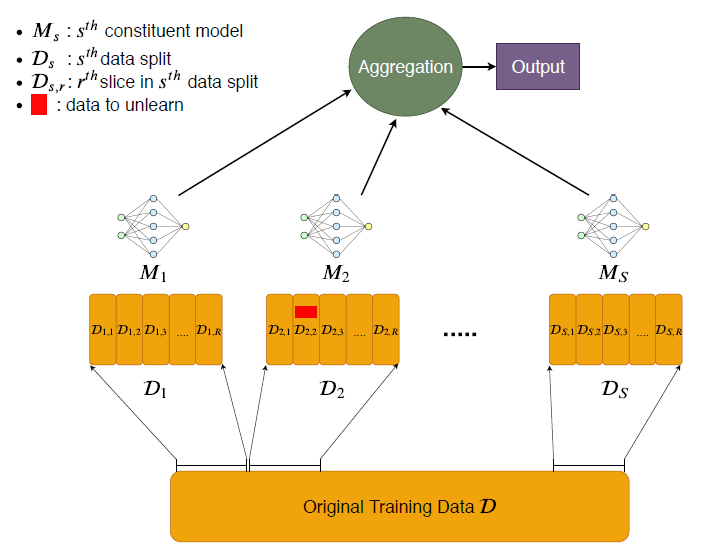
\includegraphics[width=0.9\linewidth]{machine_unlearning.png}
    \caption{将数据集分成若干互不相交集合分别训练}
    \label{fig:machine_unlearning}
\end{figure}
\begin{figure}
    \centering
    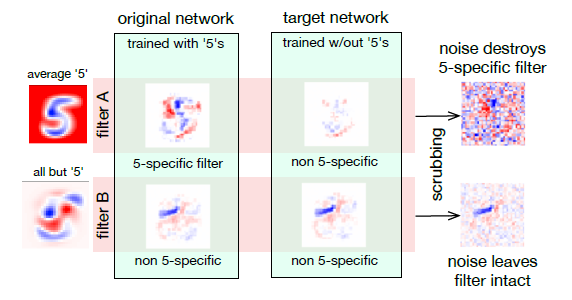
\includegraphics[width=0.9\linewidth]{eternal_sunshine.png}
    \caption{将数据集分成若干互不相交集合分别训练}
    \label{fig:eternal_sunshine}
\end{figure}
这篇文章\cite{Golatkar_2020_CVPR}实现了一种通过在权重上增加噪音的方法来逐渐减少神经网络参数对遗忘数据的信息量,如图~\ref{fig:eternal_sunshine}。同时提出了一些衡量遗忘效果的指标,比如遗忘集的测试准确率,保留集(没有被遗忘的数据集)的测试准确率和测试集的测试准确率。还提出了模型信心的指标,就是对比目标神经网络与此文方法遗忘之后的网络针对遗忘集和保留集输出的交叉熵。这些指标在实际应用上具有参考价值,因此本文也参考了这些评价指标。这篇文章中还提到了一种信息论领域常用到的信息边界的衡量方法,就是计算两个网络模型参数的KL散度距离(Kullback-Leibler Divergence)。这种方法经常用于量化两个随机变量概率分布的相似性。然而,遗忘的目的并不只是简单地让网络的参数去接近目标网络就可以,因此这个衡量指标没有被本文所采用。这个方法虽然在遗忘的效果上达到了较为理想的状态,然而在没有遗忘的类别的准确率上面不是很理想。
这篇文章\cite{Golatkar_2021_CVPR}提出了一种混合训练模型,将训练集分为核心训练集和用户训练集。核心训练集表示学习后不会被遗忘的训练集,用户训练集代表学习后可能会被用户遗忘的训练集。文章中使用了两个神经网络用来训练。第一个网络只用核心训练集进行训练,第二个网络使用第一个网络的输出结果和用户训练集以及核心训练及一起进行训练。当用户申请遗忘数据时,系统会根据没有被遗忘的数据集还有训练好的第一个网络的权重,计算出一个权重变化差,记为$\Delta$w。第二个网络的权重减去这个$\Delta$w即可得到遗忘之后的权重。为了使遗忘的效果更加明显,减去$\Delta$w后再加上一定方差的噪声。文章使用的指标是遗忘集、保留集和测试集的准确率,重新学习时间,激活距离,还有伙伴推断攻击的成功率。激活距离定义为目标遗忘网络和这个方法遗忘后的网络对测试集输出差的第一范数值。伙伴推断攻击的目的是对于给定一个输入,通过一些方法和手段来判断这个输入是否被用于训练网络。其准确率被这篇文章用来当作评价遗忘效果的一个指标。本文借鉴了激活距离和伙伴推断攻击准确率这两个评价指标。
\section{迁移学习的研究}
\paragraph{}这篇文章\cite{10.1007/978-3-030-01424-7_27}是一篇关于迁移学习的综述。文章中给迁移学习下的定义是给定一个数据集Dt和一个学习任务Tt,这个学习任务可以根据另外一个基于数据集Ds的学习任务Ts获得帮助,从而加快学习任务Tt的学习进程。这个概念中要解决的问题和我们面临的遗忘问题如出一辙。文中将迁移学习分为四类,即基于实例的迁移学习,基于映射的迁移学习,基于网络的迁移学习以及基于对抗的迁移学习。其中第三点基于网络的迁移学习提出了共享网络参数来加快目标网络的学习,就是将训练好的神经网络的前若干层的网络结构和参数迁移至新的神经网络,将这些网络连结和学习参数作为新的神经网络的一部分,过程如图\ref{fig:transfer_learning_1}所示。这种思想来源于对人类大脑处理信息机制的理解。神经网络和人类大脑处理信息的极致很类似,前面的层次负责提取特征,像是一个特征提取器,这些提取后的特征又会被后面的网络继续提取特征。
\begin{figure}
    \centering
    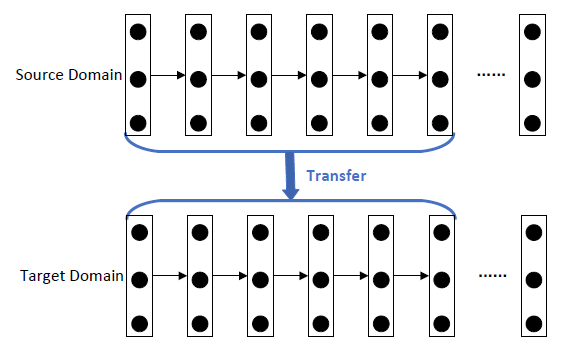
\includegraphics[width=0.9\linewidth]{transfer_learning_1.png}
    \caption{基于网络的迁移学习模型示意图}
    \label{fig:transfer_learning_1}
\end{figure}
\paragraph{}这篇文章\cite{6639081}也采用了相同的思路,实现了语音识别语言的功能。如图\ref{fig:transfer_learning_2}所示,作者将网络分成两个部分,前一部分是语言独立的特征提取器,最后一层是语言相关的分类器。神经网络的输入是不同语言的语音片段,经过共享的特征提取器,输出到最后的全连接层,从而可以达到识别语言种类的目的。文中指出,对于欧洲的四种语言,相比于使用单个语言训练的网络,单词的错误率下降了3\%-5\%。而对于英语和中文,相比于使用单个语言训练的网络,单词错误率下降了6\%-28\%。
\begin{figure}
    \centering
    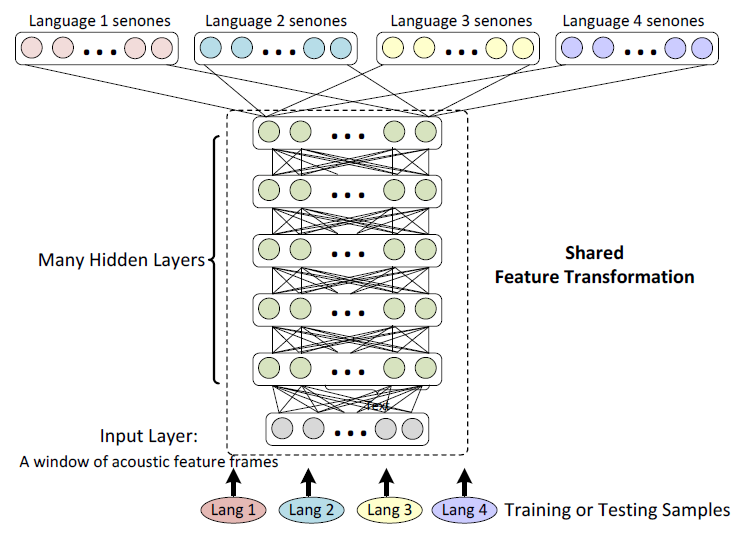
\includegraphics[width=0.9\linewidth]{transfer_learning_2.png}
    \caption{共享特征提取器的语言识别网络}
    \label{fig:transfer_learning_2}
\end{figure}
这篇文章\cite{Oquab_2014_CVPR}也讲到了共享特征提取器。如图\ref{fig:transfer_learning_5}所示,网络可以分成两个部分,一部分是卷积层,另一部分是全连接层。先将网络在一个训练集上训练,训练完成后,将卷积层和若干全连接层迁移到另外一个分类任务当中,替代网络中的卷积层和若干全连接层。为了更好地适应新的分类任务,作者新增了两层全连接层,然后使用新的训练集对网络进行训练,训练的同时冻结迁移过来的参数,只训练新增的全连接层的参数。训练至收敛后,网络同样取得了很好的效果。 
\begin{figure}
    \centering
    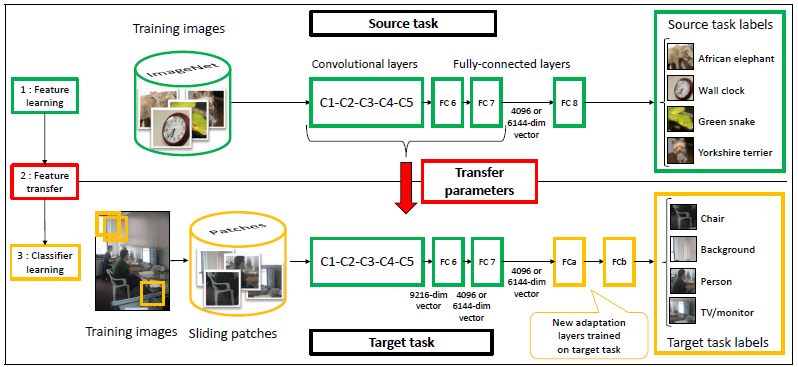
\includegraphics[width=0.9\linewidth]{transfer_learning_5.png}
    \caption{共享特征提取器的卷积神经网络}
    \label{fig:transfer_learning_5}
\end{figure}
这篇文章\cite{yosinski_2014_NIPS}对深度神经网络的特征可共享的特性进行了研究。如图\ref{fig:transfer_learning_3}所示,第一行代表用数据集1训练的网络,第二行代表用数据集2训练的网络。第三行代表将前三层参数冻结或者不冻结,并且将第二行前三层的参数迁移至第三行前三层参数。第四行代表前三层参数使用第一行训练好的前三层参数,之后的训练将这三层参数冻结或者不冻结进行训练。最终的结果如图\ref{fig:transfer_learning_4}所示,不冻结参数用不同数据集训练的网络得到了很好的泛化效果。从这个实验中可以看出,深度神经网络前若干层参数是可以共享的。
\begin{figure}
    \centering
    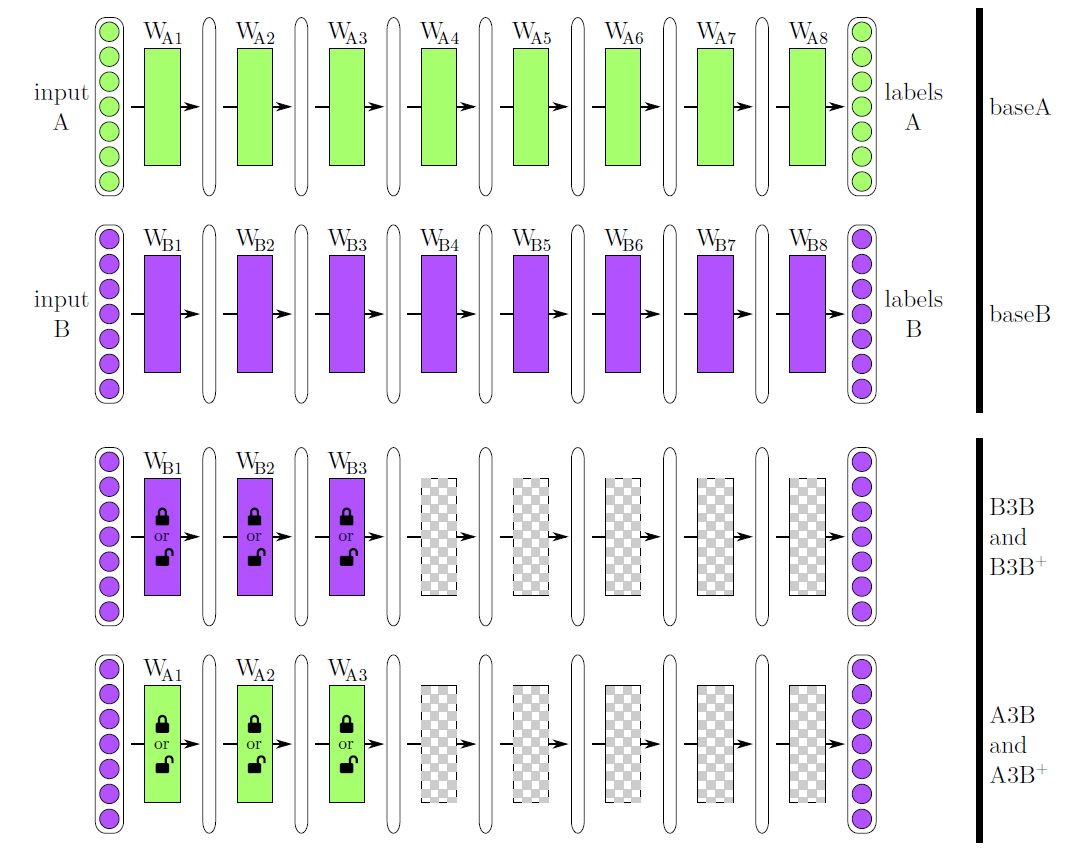
\includegraphics[width=0.9\linewidth]{transfer_learning_3.png}
    \caption{共享参数的深度神经网络训练示意图}
    \label{fig:transfer_learning_3}
\end{figure}
\begin{figure}
    \centering
    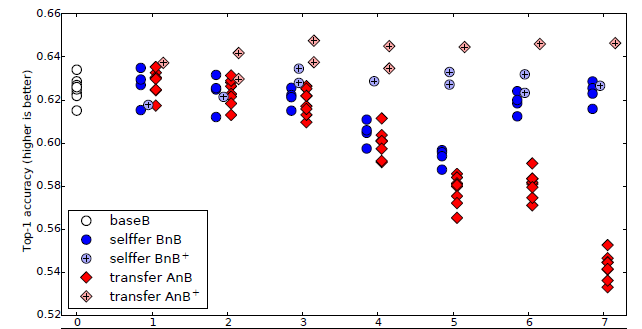
\includegraphics[width=0.9\linewidth]{transfer_learning_4.png}
    \caption{共享参数后实验结果}
    \label{fig:transfer_learning_4}
\end{figure}

\section{增强学习的研究}
增量学习\cite{PARISI201954}是指已经学习完成的机器学习模型继续学习新的数据的技术。增量学习遇到的挑战是灾难性遗忘,在已经学习完成的机器学习模型上只用新的数据集去训练会出现以前学习过的分类准确率出现下降的现象,就好像学习了新的知识将旧的知识忘记了。为了克服灾难性遗忘,这篇综述中提到增强学习大致可分为三种类型:基于正则化的方法,基于动态结构的方法以及基于补充学习系统(CLS)和记忆重放的方法。
增量学习的研究中,这篇文章\cite{8107520}是一篇具有代表性的文章。如图\ref{fig:incremental_learning_1}所示,图中展示了一个已经学习完成的网络在遇到新的学习任务时可能的学习方法。(a)中是原来已经学习好的模型,前半部分是卷积神经网络,后半部分是全连接层。当加入一个新的类别后,大概有三种可能的解决方法。一种是微调(fine-tuning),即在原来的网络上用新的训练数据直接训练。这样的方法会毫无疑问导致灾难性遗忘。第二种方法是联合训练(Joint Training),就是用新的训练数据和旧的训练数据同时训练原有的网络,这样带来的效果是比较好的,但是重新训练的成本是很大的。第三种方法是特征提取(Feature Extraction)的方法。和以前训练好的网络分享一部分参数,这部分参数不用来更新。然后用新的训练数据继续训练没有被冻结的参数。这样的方法可能的问题是新的训练数据的特有的特征无法被原有网络提取,因此最终的效果也不会很好。然而,遗忘和增量学习不同的是,遗忘学习是在原有的模型上做减法,所以不会涉及到新数据有特有特征的问题。
\begin{figure}
    \centering
    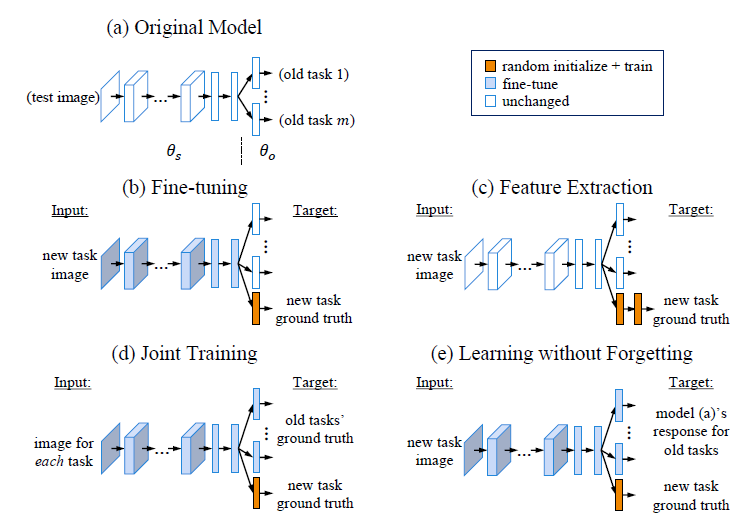
\includegraphics[width=0.9\linewidth]{incremental_learning_1.png}
    \caption{增量学习可能的方法分类}
    \label{fig:incremental_learning_1}
\end{figure}
这篇文章\cite{Sarwar_2020}通过共享网络层次,建立新网络分支来解决灾难性遗忘的问题。如图\ref{fig:incremental_learning_2}所示,原来的网络已经训练了50个类别,当有10个新的类别需要添加到网络中时,确定好共享网络,然后冻结共享网络和原来网络的网络参数,只用新的训练数据对新增加的网络进行训练。当需要做预测时,将两个网络的输出综合起来,判断应当输出的结果。这样的网络随着新增的类别不断增多而逐渐增大。但是我们可以看到共享网络参数的思想。
\begin{figure}
    \centering
    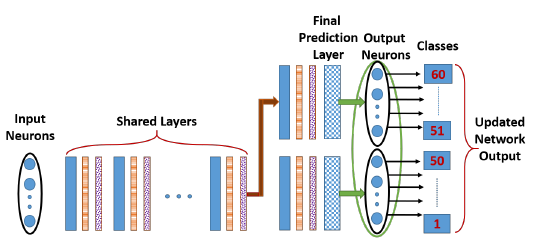
\includegraphics[width=0.9\linewidth]{incremental_learning_2.png}
    \caption{共享网络参数的增量学习}
    \label{fig:incremental_learning_2}
\end{figure}
\section{本章小结}

%% !TeX root = ../thuthesis-example.tex

\chapter{卷积神经网络的分层抽象特性和遗忘方法}
上一章阐述了遗忘学习的研究现状和和遗忘学习相关的研究工作。本章的主要内容是介绍卷积神经网络的一个重要特性,即分层抽象特性。为了让读者能够更好地理解卷积神经网络的分层抽象特性,我们将首先介绍卷积神经网络的工作原理以及设计思想。接下来再介绍基于卷积神经网络分层抽象特性的遗忘思想以及遗忘方法。最后将介绍评价遗忘的性能指标。

\section{卷积神经网络的介绍}

\subsection{卷积神经网络的结构}

首先,我们看卷积神经网络的网络结构,大致了解卷积神经网络的框架。卷积神经网络和多层感知机的神经网络很类似,它们都可以通过像堆积木一样来组装构建。然而,卷积神经网络里和多层感知机不同的是出现了Convolution 层(通常称为卷积层)和Pooling 层(通常称为池化层)。

下一小节会详细介绍卷积层与池化层,在这我们首先看如何将各层组织起来构建卷积神经网络。基于多层感知机的神经网络中,相邻层的各个神经元之间都有连接,这样的结构被称为fully-connected(通常称为全连接)。Pytorch工具中已经实现了全连接层。如果使用全连接层来搭建网络,我们可以通过如图\ref{fig:chapter3_3}所示的神经网络结构实现一个五层的简单神经网络。
如图\ref{fig:chapter3_3}所示,在使用全连接层搭建的神经网络中,全连接层后面直接跟着激活函数ReLU(或者Sigmoid)。这里使用了4 层全连接和ReLU的组合,接着的第5层是全连接层,最后一层则是Softmax层,输出最终的预测结果。
\begin{figure}
    \centering
    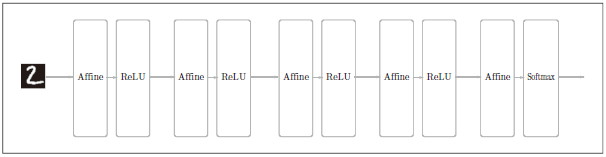
\includegraphics[width=0.9\linewidth]{chapter3_3.png}
    \caption{全连接网络结构示意图\cite{luyujie_202}}
    \label{fig:chapter3_3}
\end{figure}
如图\ref{fig:chapter3_2}所示,这就是一个卷积神经网络的例子。
\begin{figure}
    \centering
    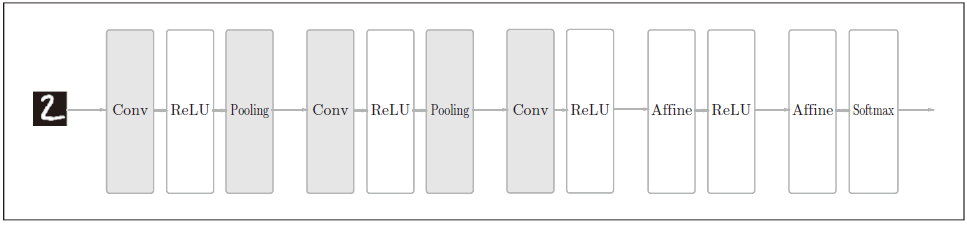
\includegraphics[width=0.9\linewidth]{chapter3_2.png}
    \caption{卷积神经网络结构示意图\cite{luyujie_202}}
    \label{fig:chapter3_2}
\end{figure}
如图\ref{fig:chapter3_2}所示,卷积神经网络中增加了卷积层和池化层。卷积神经网络的单个层连接的顺序是卷积层,激活函数层和池化层,其中池化层有时可以省略。这样的组合方式可以被理解为前面的全连接层和激活函数层组合连接被替换成了卷积层,激活函数层和池化层的连接。另外,在如图所示的卷积神经网络中,靠近后面的输出层中使用了全连接层和激活函数层ReLU组合。然后,最终的输出层中则使用了全连接层和Softmax的组合。这样的搭配一般都是卷积神经网络中较为常见的搭配结构。
\subsection{卷积神经网络的原理}
在全连接的神经网络中,各个层次都是通过全连接层来组织起来的。在全连接的层次中,各个神经元都是连接在一起的,全连接的网络的输出数量是可以任意指定的,没有数量上的限制。

这样的结构会带来一定的问题,那就是数据的形状特征没有被充分地利用起来。用图片来举例,神经网络输入图片时,图片数据的格式一般是长、宽和高。长和宽代表图片像素点的长度和宽度,高代表图片采样通道的宽度。然而,这样的数据结构输入到全连接层搭建的神经网络中时,就会被拉长为一维的数据。举例说明,MNIST的数据集中一张图片的长是28个像素点,宽是28个像素点,高度是1个通道(图片用黑白表示)。这样的形状输入到全连接的网络中前会被展开成一列,就是784个数据点输入到网络中。按照常识可以知道,图片一般是三维的形状。

这样的形状结构中包含重要的空间位置关系信息。比如通道与通道之间的关联信息,空间上相互距离比较接近的像素点一般具有相似的值,距离比较远的像素点一般没有关联,因此三维形状的数据中可能会蕴藏很多可以挖掘的特征模式。全是全连接层的神经网络就会把数据拉长成一维数据,从而没有充分利用图片中的空间位置信息。

卷积神经网络就不会这样,图片输入到网络中就是以三维数据的格式输入,一个卷积层处理好数据以后,让然会以三维的格式输入到下一个卷积层中。所以,卷积神经网络对于理解图像这样带有空间位置信息的数据是很有优势的。
\subsubsection{卷积层}
卷积运算发生在卷积层,卷积运算的计算过程类似滤波处理过程。因此用于卷积运算的卷积核有时又被称为滤波器。常规的卷积运算如图\ref{fig:chapter3_4}所示。图中展示的便是一次二维卷积运算的过程。输入数据的尺寸是4乘4,卷积核的尺寸是3乘3,没有边界填充的情况下,最终输出结果的尺寸是2乘2。
\begin{figure}
    \centering
    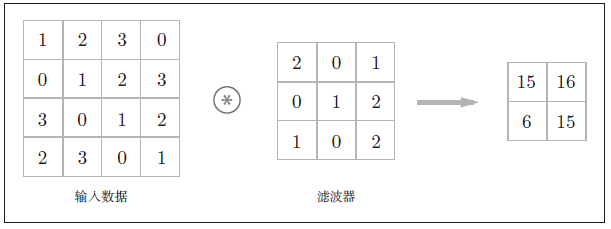
\includegraphics[width=0.9\linewidth]{chapter3_4.png}
    \caption{简单的卷积运算\cite{luyujie_204}}
    \label{fig:chapter3_4}
\end{figure}
卷积运算的具体过程是什么样的呢?下面结合图片\ref{fig:chapter3_5}来具体说明。如图\ref{fig:chapter3_5}中的第一行所示,第一行灰色区域代表第一步卷积操作所发生的区域,这个区域内的数字和卷积核的形状是相同的,所以区域内的数字可以与卷积核中对应位置的数字相乘,然后再把这些相乘的结果相加就得到了第一个结果,运算后将结果保存到相应的位置。如图\ref{fig:chapter3_5}第二、三、四行所示将上面讲的过程在每个位置计算一遍,于是就完成了一次卷积运算。
\begin{figure}
    \centering
    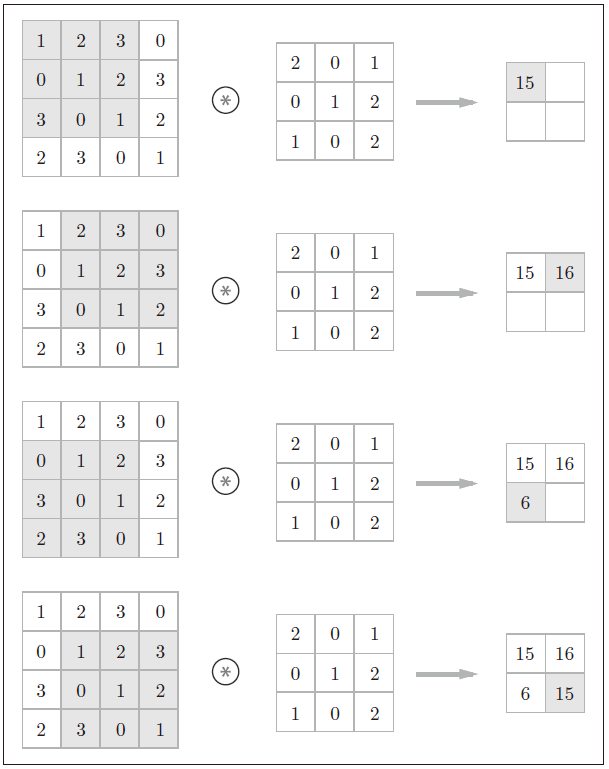
\includegraphics[width=0.9\linewidth]{chapter3_5.png}
    \caption{卷积运算过程示意图\cite{luyujie_205}}
    \label{fig:chapter3_5}
\end{figure}
和全联接的网络相同,除了网络的权重之外,还有偏置。卷积神经网络中偏置的个数一般是卷积核的个数,而且每个卷积核对应的偏置的维度一般是1乘1。计算完卷积之后,在相应结果的每个位置再加上偏置数字便得到了最终输出的数据,其计算过程如图\ref{fig:chapter3_6}所示。对于输入数据,滤波器(维度是3*3)与输入数据(维度是4*4)进行卷积元算后便得到了初步的输出结果(维度是2*2),之后再将这个结果的每一个位置加上该卷积核对应的偏置数值,得到了最终结果(维度是2*2)。
\begin{figure}
    \centering
    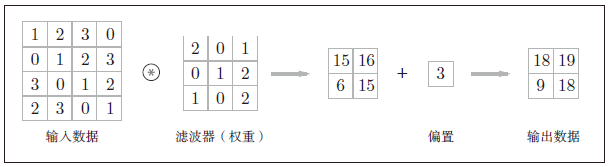
\includegraphics[width=0.9\linewidth]{chapter3_6.png}
    \caption{卷积运算后的偏置\cite{luyujie_206}}
    \label{fig:chapter3_6}
\end{figure}
三位卷积运算与二维卷积运算不同的是,卷积核的维度从2维提高到了3维,除了有长和宽的信息,还有通道数的维度。如图\ref{fig:chapter3_7}所示,以3通道为例,其运算过程与二维相似,现将对应位置的数字相乘,然后将相乘之后的结果相加,便得到了输出结果。
\begin{figure}
    \centering
    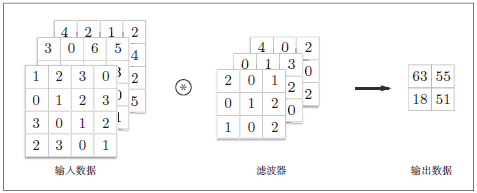
\includegraphics[width=0.9\linewidth]{chapter3_7.png}
    \caption{加上边界填充的卷积运算\cite{luyujie_206}}
    \label{fig:chapter3_7}
\end{figure}
\subsubsection{池化层}
为了减少参数的数量,提高神经网络泛化能力,在卷积伸进网络进行卷积运算以后,通常会进行池化操作。池化操作会同时减少卷积操作结果的长度和宽度。其运算过程如图\ref{fig:chapter3_8}所示。在第一行,图中灰色区域就是池化操作的一个操作单元,这个操作单元的大小来自池化操作的输入参数。池化操作的输入是图中灰色区域内的数字,输出是一个数字。中间的运算过程一般有两个算法,一种是去所有数字中最大的数字,这种算法一般被称为最大池化操作;另外一种算法是取区域内所有数字的平均数,这种算法一般被称为平均池化操作。
\begin{figure}
    \centering
    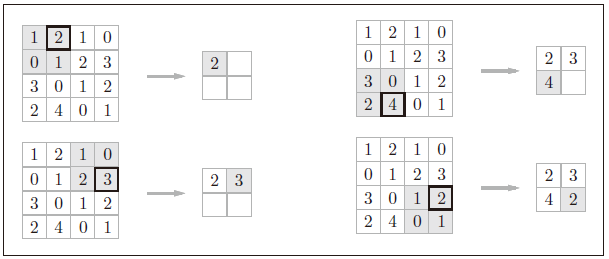
\includegraphics[width=0.9\linewidth]{chapter3_8.png}
    \caption{池化操作流程图\cite{luyujie_214}}
    \label{fig:chapter3_8}
\end{figure}
池化层与卷积层不一样的是,池化层没有训练参数,它的输入参数都是运算之前系统已经规定好的。池化层就是一个固定算法的函数。它另外一个特点是,池化操作后通道数是不变的,各通道是相互独立的,如图\ref{fig:chapter3_10}所示。
\begin{figure}
    \centering
    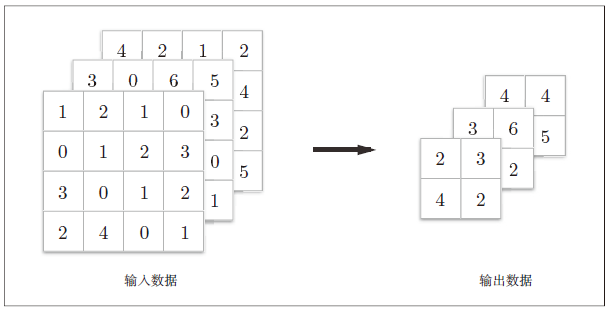
\includegraphics[width=0.9\linewidth]{chapter3_9.png}
    \caption{三维数据的池化操作\cite{luyujie_215}}
    \label{fig:chapter3_9}
\end{figure}
加入池化层后,神经网络对输入数据发生的一些微小干扰噪声具有很好的鲁棒性。如图\ref{fig:chapter3_10}所示,即使图片发生了微小偏移,经过池化操作后,其特征仍能被准确地识别出来。
\begin{figure}
    \centering
    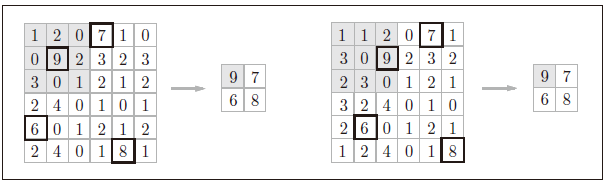
\includegraphics[width=0.9\linewidth]{chapter3_10.png}
    \caption{池化操作对发生偏移的输入具有鲁棒性\cite{luyujie_216}}
    \label{fig:chapter3_10}
\end{figure}
\section{卷积神经网络的分层抽象特性}
\subsection{人类视觉信息处理原理}
1981年来自美国的科学家David Hunter Hubel和来自瑞典的科学家Torsten Wiesel被授予了诺贝尔生理学或医学奖,以表彰他们研究人类视觉系统信息加工领域作出的杰出贡献。他们在人类视觉系统信息加工领域的工作贡献了当今神经生物学教科书视觉部分的一半内容,成为所有研究神经生物学方向学生的必学内容,这篇回忆录\cite{Hubel1998EarlyEO}中记录他们一起共事的过程。在他们的这篇工作\cite{https://doi.org/10.1113/jphysiol.1959.sp006308}中记录了麻醉后的猫的大脑对不同视觉光斑刺激的反应,并记录下了视觉皮层神经元的活动。
如图\ref{fig:chapter3_11}所示,他们在实验中发现,有一类细胞对一定范围视野内特定朝向上的刺激反应强烈,他们称这样的现象为朝向选择性,称这样的细胞为简单细胞。这样的细胞仅对狭窄的视觉感受野有反应,刺激他们最好的方式就是比较狭长的光斑,而且刺激的产生有明显的边界,当光斑覆盖整个作用区域时,并不能产生刺激反应。因此这样的细胞被看作是专门用来感受线条或边缘的信号接收器。他们通过进一步的实验发现,还有一类细胞,虽然对特定方向光斑的刺激有强烈反应,但是并没有明显的感受野。他们发现这样的细胞的上游是许多简单细胞,接受简单细胞发过来的刺激信号。他们称这样的细胞为复杂细胞。这种模式可以理解为复杂细胞是简单细胞的抽象,猫的视觉系统具有层级结构,图\ref{fig:chapter3_12}展示了简单细胞和复杂细胞的关系。
\begin{figure}
    \centering
    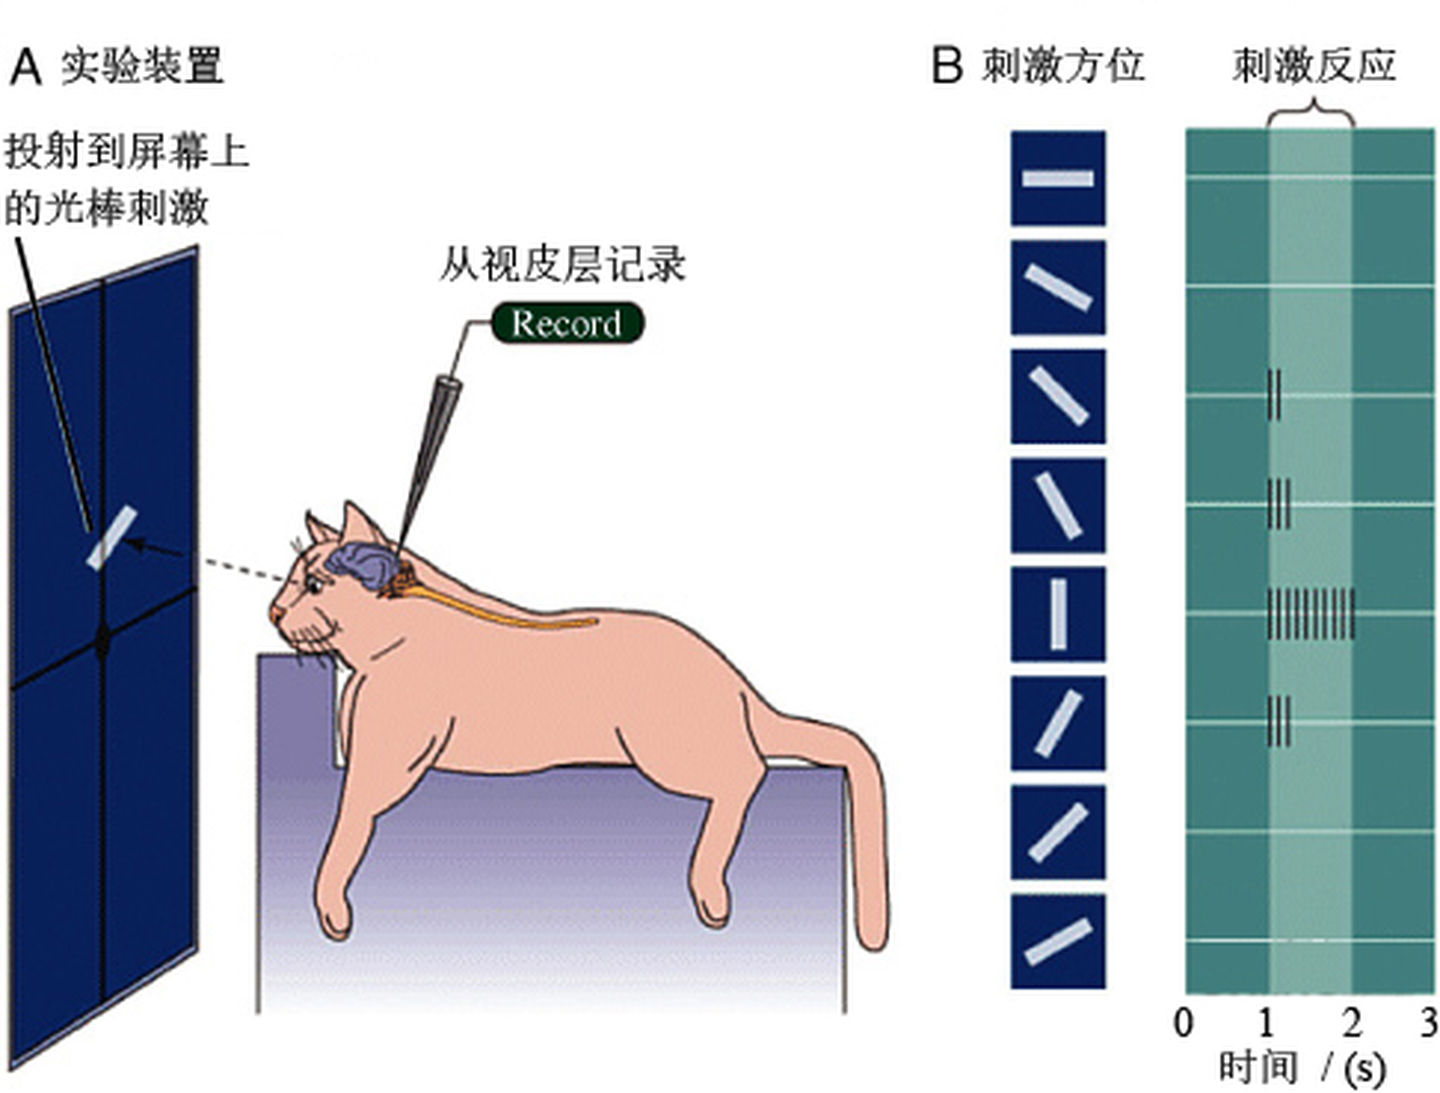
\includegraphics[width=0.9\linewidth]{chapter3_11.jpeg}
    \caption{使用光斑刺激猫的视神经,并记录猫的神经反应\cite{yanjianweishi}}
    \label{fig:chapter3_11}
\end{figure}
他们这样的发现对理解人类视觉信息加工过程很有帮助。首先人类的视网膜接收外界传入的信号,经过简单细胞处理后,简单细胞完成了一些初级特征的提取,比如简单的直线或边缘的信息。简单细胞后面有复杂细胞,复杂细胞负责完成更为抽象层次信号的处理,比如由各种方向的直线或边缘组成的形状的信息,比如三角形或正方形等。复杂细胞上面的细胞负责处理更为抽象的信息,经过一系列信息的抽象后,人类大脑就能识别看到的图像是一个什么物体。因此人类视觉信息加工是一个不断将信号进行抽象处理的过程。
\begin{figure}
    \centering
    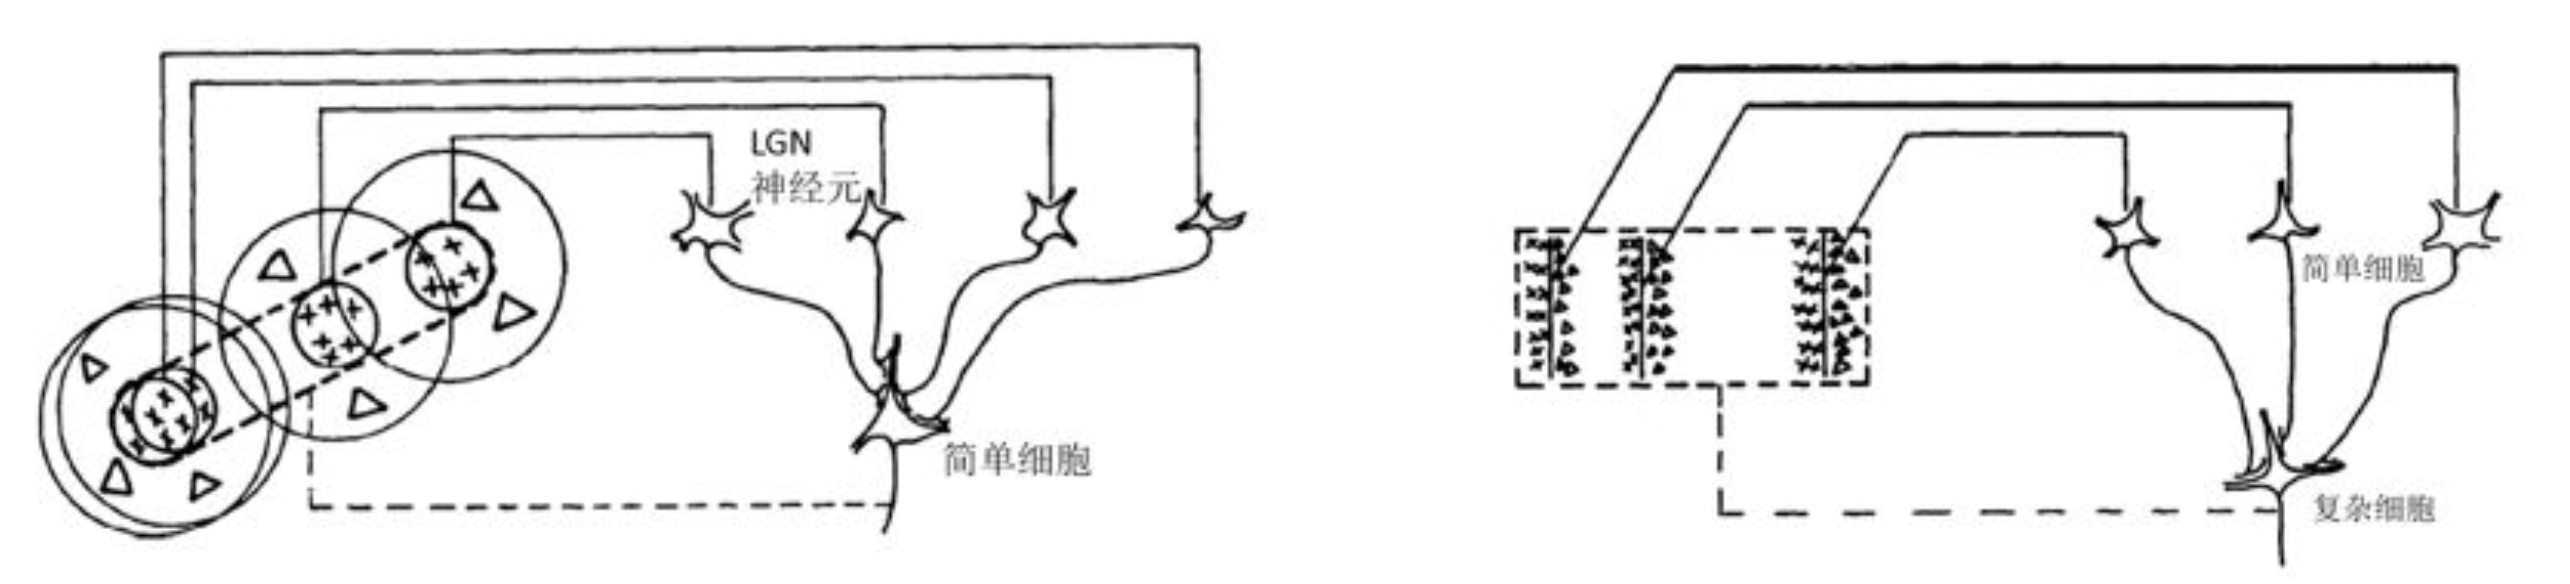
\includegraphics[width=0.9\linewidth]{chapter3_12.png}
    \caption{人类视觉信息处理过程中的简单细胞与复杂细胞\cite{yanjianweishi}}
    \label{fig:chapter3_12}
\end{figure}

\subsection{卷积神经网络的分层抽象特性}
在这篇文章\cite{2019arXiv190906161K}中,作者提到了卷积神经网络是最接近还原人类视觉信息加工原理的人工神经网络。从本章第一节讲到的卷积神经网络的基本原理中可以知道,卷积神经网络中的卷积核在与输入数据进行卷积操作时,很类似人类视觉感受野中的朝向选择性。随着输入数据在多层卷积层中逐层传递,使得一些特征信息逐渐被卷积核提取,提取的信息也逐步抽象。本文将卷积神经网络这种区别于其他人工神经网络的特性称为卷积神经网络的分层抽象特性,层数较低的卷积核提取的是较为初级的基本特征,层数越高的卷积核提取的特征越抽象。如图\ref{fig:chapter3_13}所示, 图中上半部分展示了一个优化完成的8层卷积神经网络结构。下半部分则是参数渲染后的效果。我们可以看到第一个卷积层学到的信息是一些基础的信息,例如边和角;第三层学到了由边和角构成的图案;第五层则学到了由图案构成的物体的某个部分;最后,全连接层学到的是整个物体本身。由此可以看出在卷积神经网络模型中,越靠后面的层次往往是前面层次的抽象(这里我们称离输入端较近的层次为前面层次,离输入端较远的层次为后面层次),这种现象就解释了我们所说的分层抽象特性。
\begin{figure}
    \centering
    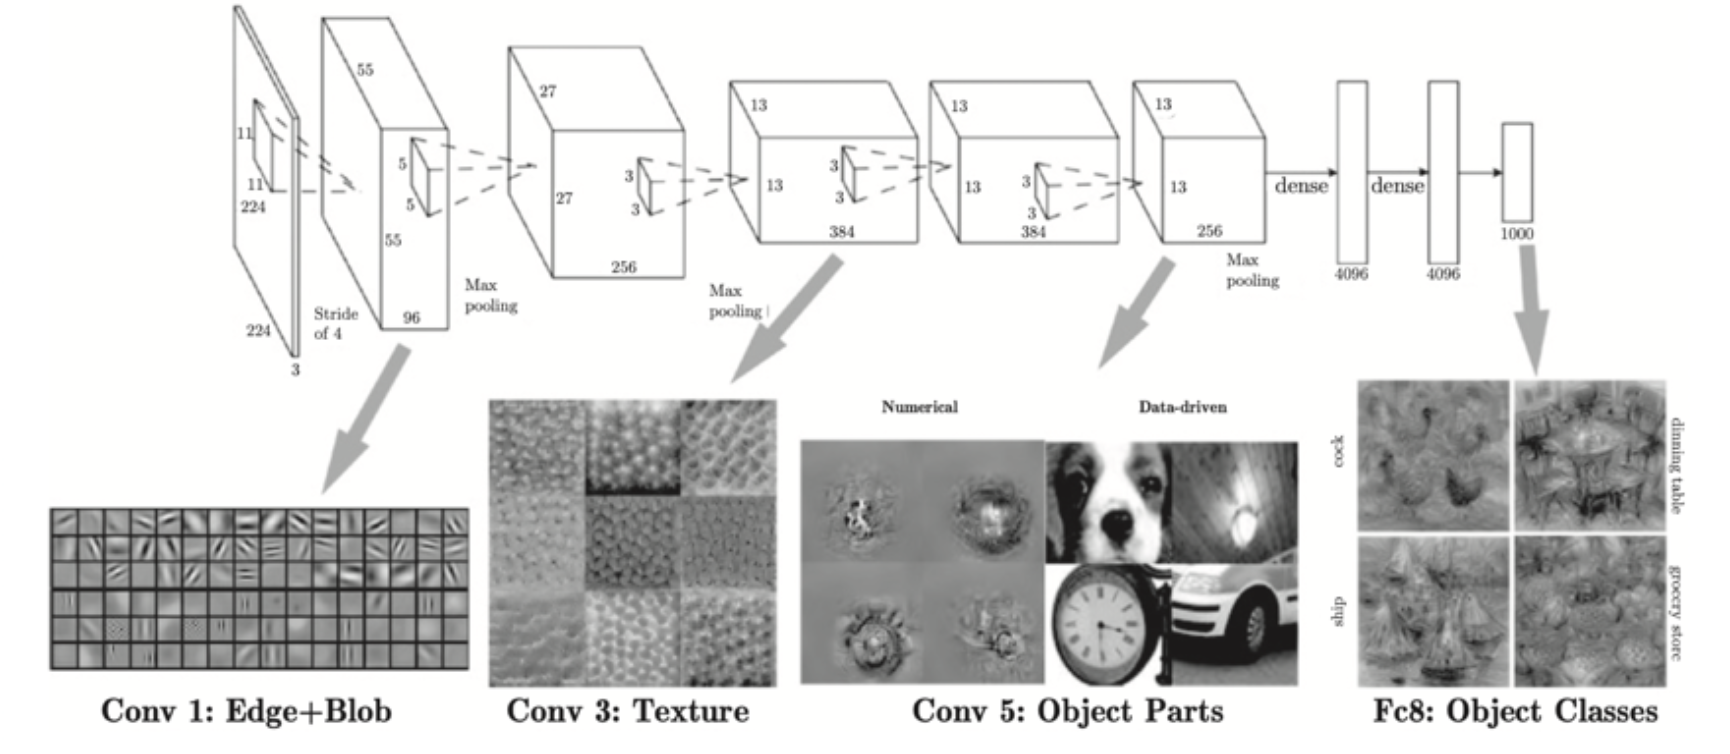
\includegraphics[width=0.9\linewidth]{chapter3_13.png}
    \caption{卷积神经网络的分层抽象特性示意图\cite{luyujie2018}}
    \label{fig:chapter3_13}
\end{figure}

\section{基于卷积神经网络的遗忘方法}
\subsection{遗忘方法的思路介绍}
我们首先来讨论什么是遗忘。理想的遗忘效果是就好像一个神经网络模型从来没有使用遗忘数据训练过一样。换一个角度考虑,一个用户之所以会选择让模型遗忘自己的数据,其初衷是出于保护个人隐私。因此遗忘的目的就是为了防止模型攻击造成信息泄露当前的攻击方法有多种多样,我们无法也不可能去针对每种攻击方法去设置防御方法。我们能做的就是消灭信息,换句话说,消灭的信息越多,攻击者得到的信息就越少。消灭信息的极限就是重新训练。然而重新训练的代价是十分巨大的,一个神经网络模型少则几千个参数,多则高达数亿参数,重新训练的代价是十分昂贵的。所以完全消灭所有信息看起来是不现实的。
那么有没有一种折中方案,既可以消灭信息,又能不用重新训练付出那么多代价?答案是肯定的,那就是我们不用消灭所有的信息,只消除一部分抽象信息,一些基本的信息是分类无关的,攻击者即使拿到也没有用途。这就用到了卷积神经网络特有的分层抽象特性,像人类视觉信息处理过程一样,卷积神经网络较低层次的卷积层只提取了较为基本的视觉元素,比如边、角、简单的条纹等等。随着网络层次的提高,抽象程度逐渐提高,卷积核的感受野也逐步扩大,从而能提取到更为抽象的信息,比如一些有固定模式的组织,图案等。到卷积神经网络比较高的层次后,感受野进一步扩大,从而能提到跟分类息息相关的本质特征,比如不同人脸的区分,以及不同物体的区分,如猫和狗,飞机和卡车等。
想一想,一个攻击者最希望获得哪一部分的信息呢。毫无疑问是和分类有关的本质特征信息,而不是那些比较基本的边和角的信息。沿着这个思路,于是我们就想出了一个可以既可以消灭信息,又能不用全部参数参与训练的折中方案,那就是消灭层数较高层次的参数。
消灭参数之后会带来一个问题,我们不仅消灭了要遗忘数据的较高层次的抽象信息,同时也消灭了没有被遗忘数据的较为重要的分类信息。为了解决这个问题,我们想到了用重新训练的方法。这里说的重新训练不是指要训练所有的网络参数,而是只训练我们前一步骤消灭的参数,目的是恢复那些没有被遗忘类别的高层次的信息。这一步骤我们的做法是使用没有被遗忘类别的训练数据去训练这一部分参数。
等待模型收敛之后,我们就可以得到消除了遗忘类别高层次抽象信息,同时保留了未被遗忘类别的分类信息。
\begin{figure}
    \centering
    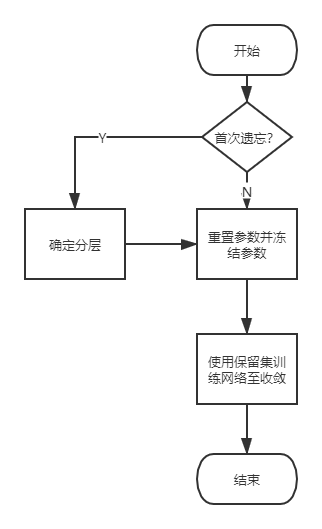
\includegraphics[scale=0.35]{chapter3_14.png}
    \caption{遗忘方法流程图}
    \label{fig:chapter3_14}
\end{figure}
遗忘方法的流程如图\ref{fig:chapter3_14}所示,

\subsection{确定分层}

前面小节讨论了遗忘方法的思路方案。随之而来的问题就是,我们需要要重置一定层数的网络参数,我们究竟要重置多少层呢?重置层数的多少直接影响了遗忘效果的好坏以及重新训练的时间,因此确定分层数量是本方法的一个重要环节。

为了确定重置参数的层数,我们要综合考虑评价遗忘效果的各个指标。首先我们要考虑在哪一层重置参数并训练后可以在遗忘集上达到较低的准确率,并且在保留类别上达到较高的准确率。考虑这个指标的因素是初余实际应用的考虑,因为我们训练神经网络模型需要神经网络对要分类的类别具有较高的准确率。然而我们有需要将要遗忘的类别很好的遗忘掉,所以我们不希望遗忘的类别具有较高的准确率。
另外一个需要考虑的因素是重新训练的时间,这也是本文存在的意义。机器学习的遗忘一个很朴素的方法就是重新训练。本文利用了卷积神经网络的分层抽象特性,使得不用完全重新训练即可达到与重新训练相近的准确率。因此,重新训练时间也是一个很重要的考虑因素,即选择的重置参数的层次并且训练后,网络收敛的时间不能太长。
还有一个很重要的指标就是训练后与完全重新训练网络的激活距离,这个距离越近越好。关于激活距离(公式\ref{index_distance})的定义会在本章的后面章节详细介绍。

有了上述确定分层的指导原则,我们就可以对分层方法进行评价。在本遗忘方法的使用过程中,是在每次执行遗忘算法的时候都需要分层一次吗?答案是否定的,我们无需在每次遗忘时均评价一次分层效果。对同一个网络结构,同一套网络训练数据集,我们仅需在首次遗忘时进行分层效果的测试,在后续的遗忘训练时,只需要使用首次遗忘时使用的分层数即可。

\subsection{重置并冻结参数}

对于重置并冻结参数的原因,在本章一开始的本方法的思路来源中已经得到了解释,是为了更好地消灭待遗忘数据在原网络中的信息。对于重置和冻结参数,我们将它们分开进行解释。
对于重置参数,我们首先考虑到的问题是,将原来需要重置参数的层次删除后,补充什么参数进去,这涉及到参数初始化的过程,也是很重要的一步。关于参数初始化有很多相关的研究成果,为了避免研究方向走偏,本文尚未对参数初始化这一变量进行系统性地研究。
我们反过来看对参数应当如何初始化,如果初始化的参数不正当,又会给我们的研究带来很大的麻烦,比如使得模型无法收敛,或者无法达到全局最优等。为了防止这样的由于参数初始化不当而带来的问题,我们选取的策略是,保存模型初始化参数,当网络中某些层次需要重置参数时,我们将保存下来的相应层次的网络参数补充到需要重置参数的层次当中。这样做的一个出发点是,既然这个网络模型初始化参数能够使得网络达到收敛状态,就说明这个参数是一个较为合理的初始化参数,没有均值过大或过小,或方差过大或过小的异常情况。经过实验证明,这种做法具有一定的合理性,在实验中并未发现由于重置参数不当而带来的网络训练无法收敛的问题。

对于冻结网络,我们需要关注的问题是冻结网络的必要性方面,即到底需不需要冻结网络。对于这个问题,前人已经有人做了一定的研究工作。

在这篇文章\cite{yosinski_2014_NIPS}中,作者设置了对比实验。如图\ref{fig:transfer_learning_3}所示,图中的第一行和第四行与本文无关。图中的第二行代表一个8层的卷积神经网络使用训练集B进行训练,得到baseB。第三层代表将卷积神经网络的后五层参数重置,并且将前三层网络参数分别进行冻结实验和非冻结实验。冻结实验得到的网络参数称为BnB,非冻结实验得到的网络参数称为BnB+。其中n代表进行冻结和非冻结实验的网络层数。如图所示,图中将前三层网络参数进行了冻结和非冻结对比实验。因此得到的网络参数分别为B3B和B3B+,B3B是冻结参数得到的网络参数,B3B+是非冻结参数得到的网络参数。实验所用到的训练数据均为训练集B。

实验结果如图所示,selffer BnB和selffer BnB+标记为冻结参数实验得到的测试准确率和非冻结参数实验得到的测试准确率。baseB代表原训练完成网络测试准确率的大小,在这里作为参照。图中的横轴代表参与冻结实验的网络层数,和n的定义相同。结果展示了在冻结和非冻结实验中,非冻结参数的训练结果普遍好于冻结参数的训练结果,比如4层和5层。冻结其他层数时,冻结参数与非冻结参数的准确率结果相差不大。

是否冻结参数对本方法的最终效果影响较大。因为这不仅涉及到训练之后模型的准确率,也涉及到训练过程的收敛时间问题。上面的实验并没有涉及到收敛时间。为了探究是否需要冻结参数的问题,本文也设计了专门冻结参数与非冻结参数训练的对比实验。具体实验过程和结果将在本文第四章集中展示。

\subsection{训练网络}

对于重新训练网络,使用的数据集是原来的数据集减去要遗忘类别的数据集。因为是原数据集和遗忘数据集的差集,为了便于表达,以下称之为保留集。重新训练网络的目的已经在前文有所说明。重置了一部分网络参数以后,所有的训练数据中涉及到的分类信息已经全被消灭掉了。此时网络攻击者通过网络输出来还原训练数据的信息几乎是不可嫩的。为了保证没有被遗忘的类别达到删除参数以前的效果,我们使用保留集对重置的参数进行一定程度的还原。

在重新训练网络的过程中,待更新的参数数量对比完全重新训练的参数数量,少了冻结层次的参数,因此训练网络中不需要对冻结的参数去计算梯度和更新。因此从网络参数的收敛速度上看,应当是有一些减少。为了检验训练速度能够提升多少,我们设计了对比实验,分别记录了完全重新训练所花费的时间和使用本文遗忘方法训练所需要花费的时间。

对于遗忘问题,不能忽视一个方面是遗忘可持续性问题。随着遗忘次数的增多,网络的性能和完全重新训练之间的差距是否会越来越大。为了验证这一问题,我们设计了连续遗忘对照实验。

\section{遗忘效果的衡量指标} \label{forget_evaluation_index}

了解了一些关于卷积神经网络遗忘的概念之后,我们要在量上了解遗忘到什么程度才能算是比较好的遗忘效果。为此,我们设计了一些用来评价遗忘效果的指标。这些指标可以帮助我们从各个方面了解当前网络模型的训练状态。这些指标有测试遗忘集、测试保留集的准确率,收敛时间和激活距离,下面来分别介绍。
\subsection{测试准确率}

我们都知道训练神经网络的过程中,我们不仅要利用训练数据去训练网络,为了防止训练的网络出现过拟合情况,也需要用测试集去测试训练网络的泛化成果。我们将测试集根据遗忘需求分为两个部分,仅有遗忘类别测试数据的测试遗忘集和仅有保留类别测试数据的测试保留集。使用测试遗忘集的测试结果可以反映网络对于遗忘类别遗忘程度,这个准确率越低,代表对遗忘类别遗忘越彻底。同理,使用测试保留集的测试结果可以反映网络对于保留类别的保留情况,这个测试结果的准确率越高,代表保留类别的保留效果越明显。

但是并不是保留效果越高,遗忘效果越低,遗忘的效果就越好。这两个指标只是对网络学习结果的一个参照。为了评价遗忘效果我们还要参照激活距离(公式\ref{index_distance})。

\subsection{收敛时间}

收敛时间代表从本文提到的遗忘算法用保留集进行训练开始,到网络训练损失函数输出数值小于一定限制为止,中间过程的时间称为收敛时间。收敛时间用于衡量本文遗忘方法在时间上的节约程度。

训练时间会因实验环境的不同而不同,比如实验用的CPU,内存,硬盘,显卡,网络机构和数据集等,因此它也是一个相对量。只有在保证实验环境相同的情况下才具有参考意义。

之所以会将从保留集开始训练的时刻作为起始时间,是因为下面的确定分层步骤是一次性的步骤,对于同一个网络结构,同一个数据集,确定网络分层仅在进行第一次遗忘操作时需要操作一次。重置和冻结参数操作是固定程序的操作,通过脚本即可完成,无需人工参与中间处理过程,相比训练过程的时间,这个操作的时间可以忽略。

为了配合综合指标的计算,我们也将收敛时间进行了量化,将收敛时间定义为网络训练过程中,本轮Epoch中平均的损失函数值首次下降到指定限制时所花费的Epoch数。在本文的实验中,取了三个限值,分别是0.1,0.05和0.03。

\subsection{激活距离}

激活距离是指遗忘后模型与完全重新训练模型在测试集上的平均距离。它用于衡量遗忘后模型与完全重新训练模型在网络输出结果上的相似程度。它的计算公式是
\begin{equation}
I_{distance} = {\mathbb{E}}_{x\in {\mathcal{D}_{test}}}[{\Vert softmax(f_w(x)) - softmax(f_{w_{\mathcal{D}_R}}) \Vert}_2 ] \label{index_distance}
\end{equation}

$f_w(x)$代表完全重新训练的网络的输出结果,$f_{w_{\mathcal{D}_R}}$代表使用重置冻结参数遗忘方法训练出的网络的输出结果。
它们输出结果softmax函数的差值向量的第二范数在测试集上的期望,就是激活距离。


\section{本章小结}
本章对本文所使用的遗忘方法做了系统性的描述。为了讲清卷积神经网络的分层抽象特性,本章首先介绍了卷积神经网络技术的基本原理,包括卷积操作以及卷积层和池化层的作用。
其次介绍了卷积神经网络的分层抽象特性,这也是本文所使用方法的理论依据。
再次介绍了本文所使用的遗忘方法的具体步骤。最后介绍了本文用来评价遗忘效果的主要指标。

%% !TeX root = ../thuthesis-example.tex

\chapter{遗忘方法的实现与验证}

\section{实验验证}

\subsection{实验环境介绍}
我们用到的实验设备是两台服务器,
\\cpu Intel(R) 
\\Core(TM) i9-9900K CPU @ 3.60GHz
\\Intel(R) Core(TM) i7-6700K CPU @ 4.00GHz
\\内存 32g 32g
\\硬盘 ssd ssd
\\显卡  1xNvidia Geforce 2080 3xNvidia Geforce 1080
\\操作系统 ubuntu16.04LTS ubuntu16.04LTS
\\深度学习框架pytorch
\\数据集是cifar-10,正常训练集50000张图片,测试集10000张图片。遗忘两个类别,遗忘集是从正常训练集分离出来的10000张图片,遗忘测试集2000张图片。保留训练集是指正常训练集出去了遗忘集外的数据集合。保留训练集40000张图片,保留测试集8000张图片。神经网络有Resnet18和Resnet50。
\subsection{实验设计}

\subsubsection{确定冻结层数实验}
实验一:确定冻结层数实验
\\实验目的:这个实验的目的是确定网络冻结的层次数。确定的标准是根据3.5中讲到的四个指标的综合指标。
\\实验准备:正常训练集,遗忘集和保留集,还有测试集。使用的神经网络框架是Resnet18。
\\实验过程:首先使用正常训练集去训练神经网络,直至训练集准确率收敛,获得模型1,在训练网络之前保存神经网络训练之前的网络参数,记为模型0。再使用保留集重新训练一个神经网络,获得模型2。将模型1的最后一层(全联接层)的参数替换为模型0的最后一层参数,模型1其余层数的参数不变,由此得到模型1\_reset\_fc\_before\_training。将模型1\_reset\_fc\_before\_training加载到一个新的神经网络中,使用保留集去训练这个新的网络,直至训练准确率收敛,在训练过程中保持除全连接层以外层次的参数不被更新(即冻结),得到模型1\_reset\_fc\_after\_training。将模型1\_reset\_fc\_after\_training加载到模型,分别测量并记录指标一、指标二、指标三和指标四。
\\实验结束:计算并记录综合指标计算结果。
\subsubsection{冻结必要性验证实验}
实验目的:通过本实验验证冻结较低层次的参数是否对加快遗忘训练收敛速度有一定的贡献,同时观察遗忘集集准确率、保留集准确率和测试集准确率的变化情况。
\\实验准备:数据集有正常训练集,保留集。神经网络是Resnet18。
\\实验过程:
\\1. 用正常训练集训练神经网络得到模型1
\\2. 在正常训练集训练之前保留网络参数得到模型0
\\3. 用模型0的全连接层参数,替换模型1的全连接层的参数,得到模型1\_reset\_fc\_before\_training
\\4. 用神经网络加载模型1\_reset\_fc\_before\_training,网络参数全部无需冻结,用保留集训练至训练准确率收敛,得到模型1\_reset\_fc\_after\_training
\\5. 分别记录下各个指标
\\6. 分别将神经网络从最后一层到各个层的参数重置后,重复上述3-5步骤,将全连接层替换成全连接层至各个层之间的参数
\\实验结束:计算并记录各个模型综合指标计算结果
\subsubsection{反向冻结验证实验}
实验目的:验证卷积神经网络的分层抽象特性,与正向冻结实验进行对照。
\\实验准备:数据集有正常训练集,保留集。神经网络是Resnet18。
\\实验过程:
\\1. 用正常训练集训练神经网络得到模型1
\\2. 在正常训练集训练之前保留网络参数得到模型0
\\3. 用模型0的第一卷积层参数,替换模型1的第一卷积层参数,得到模型1\_reset\_conv1\_before\_reverse\_training
\\4. 用神经网络加载模型1\_reset\_conv1\_before\_reverse\_training,除了第一卷积层外,其余层数的参数全部冻结。用保留集训练至训练准确率收敛,得到模型1\_reset\_conv1\_after\_reverse\_training
\\5. 分别记录下各个指标
\\6. 分别重置第一卷积层至最后一层全连接层参数,重复上述第3-5步骤。
\\实验结束:计算并记录各个模型综合指标计算结果
\subsubsection{遗忘可持续性验证实验}
实验目的:检验冻结重置方法随着遗忘类别数量的增多有效性的变化情况
\\实验准备:数据集有正常训练集,分别遗忘掉1-9个类别的保留集1-保留集9共9个保留集。神经网络是Resnet18。
\\实验过程:
\\1. 用正常训练集训练神经网络得到模型1
\\2. 在正常训练集训练之前保留网络参数得到模型0
\\3. 使用保留集1-保留集9分别重新训练模型,得到模型\_forget\_1\_retrain,...,模型\_forget\_9\_retrain。
\\4. 用神经网络加载模型1,然后把神经网络全连接层和6层卷积层的参数重置为模型0的相应层次的参数。
\\5. 分别用保留集1-保留集9去训练步骤4中生成的网络,训练过程中冻结除了全连接层和后6层卷积层的参数。得到模型1\_fc\_conv6\_retain\_1\_finetune,...,模型1\_fc\_conv6\_retain\_9\_finetune共9个神经网络的参数。
\\6. 5中得到的网络参数进行指标测试,并记录。
\\实验结束:计算并记录各个模型综合指标的计算结果
\section{实验结果}
\subsection{确定冻结层数实验}
\begin{figure}
    \centering
    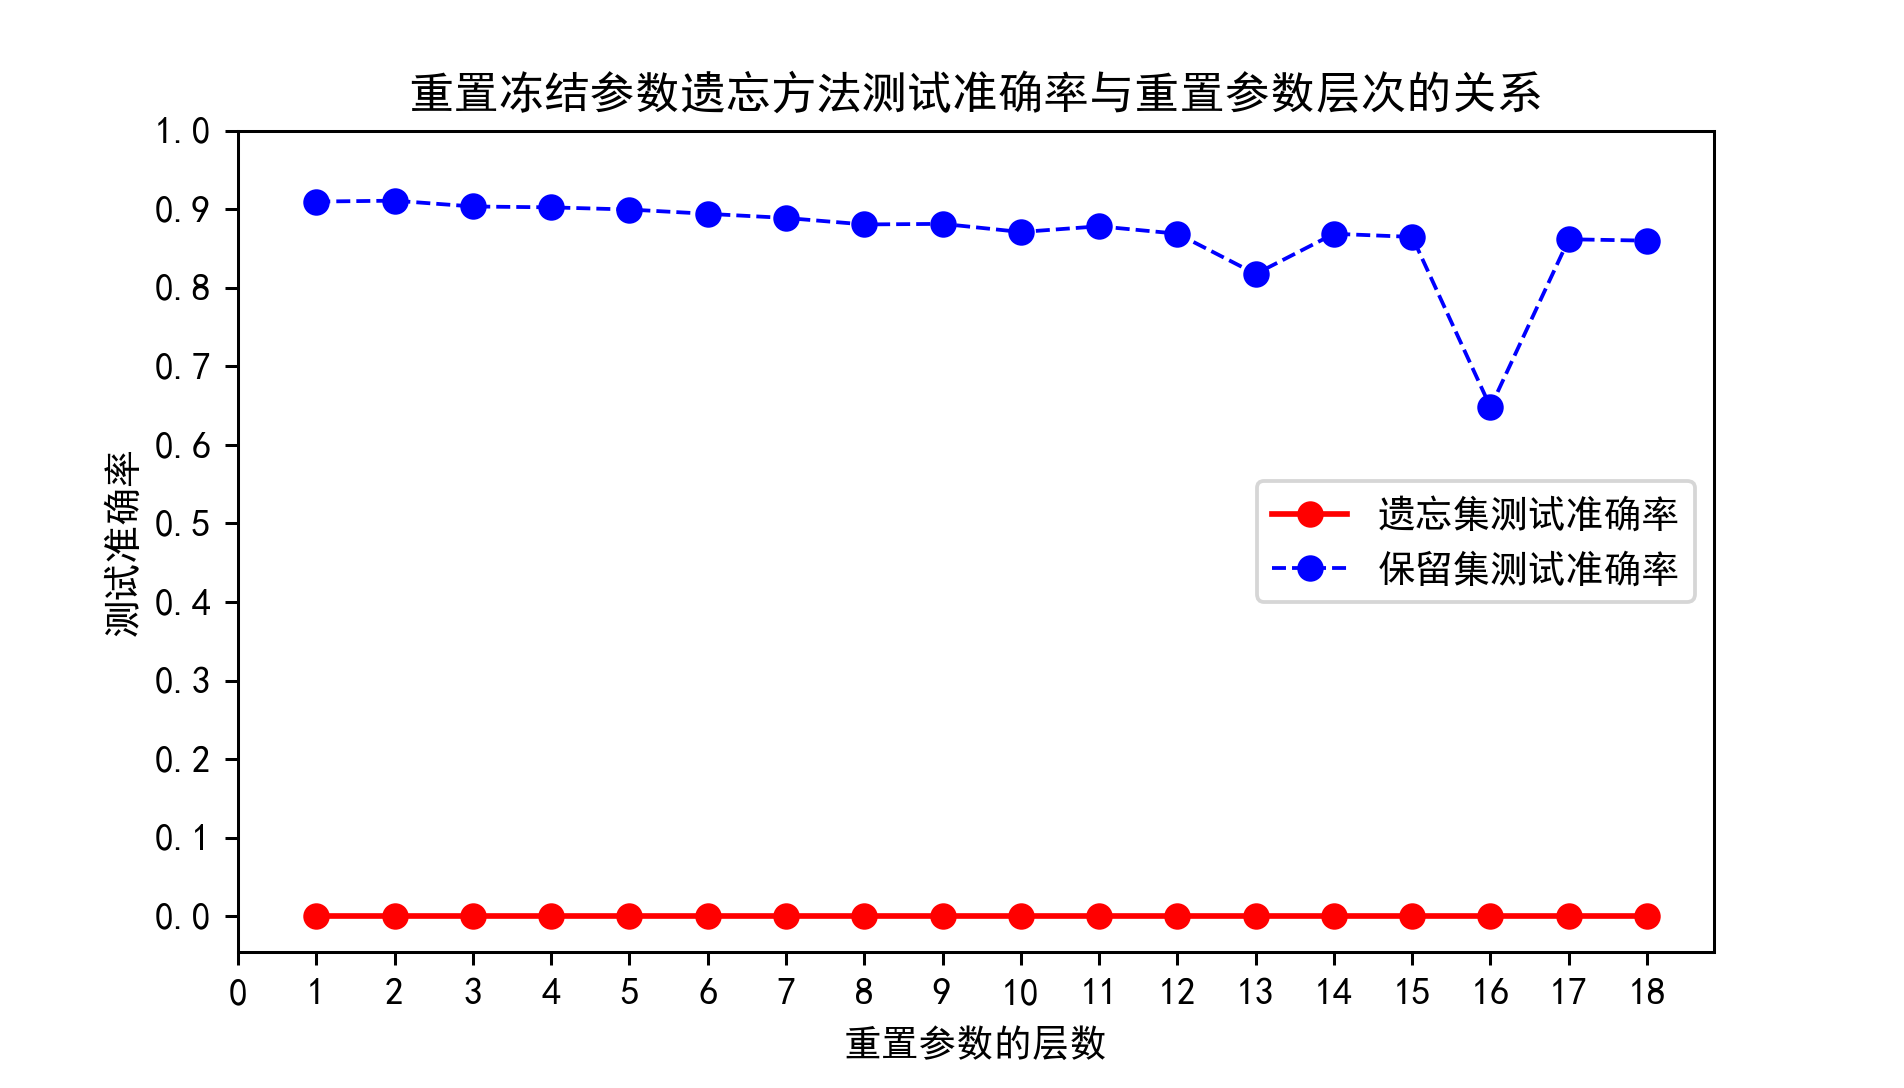
\includegraphics[width=0.9\linewidth]{chapter4_1.png}
    \caption{重置冻结参数遗忘方法测试准确率与重置参数层次的关系}
    \label{fig:chapter4_1}
\end{figure}
如图\ref{fig:chapter4_1}所示,图中展示了本文所讲述的重置冻结参数遗忘方法训练的网络用遗忘集和保留集训练之后得到测试准确率。
蓝色的折线代表利用保留测试集测试的准确率,红色的折线代表使用遗忘测试集测试的准确率的情况。
从红线可以看出,遗忘测试集的准确率全是0。这样的结果与完全重新训练得到的模型在遗忘测试集上的准确率完全相同。这说明使用本文提出的冻结重置参数方法,无论重置多少层参数,在遗忘集上均能达到理想的效果。
从蓝线与上面的点线可以看出,本方法得到的模型在保留集测试准确率上在大部分情况下均好于完全重新训练得到的模型在保留集上的准确率。
从蓝色圆点曲线中也发现随着重置参数的层数的增加,其保留集测试准确率有下降趋势,逐渐接近完全重新训练模型在保留集上的测试结果。
仅通过这一个方面还不足以让我们选出要重置参数的层次。
\begin{figure}
    \centering
    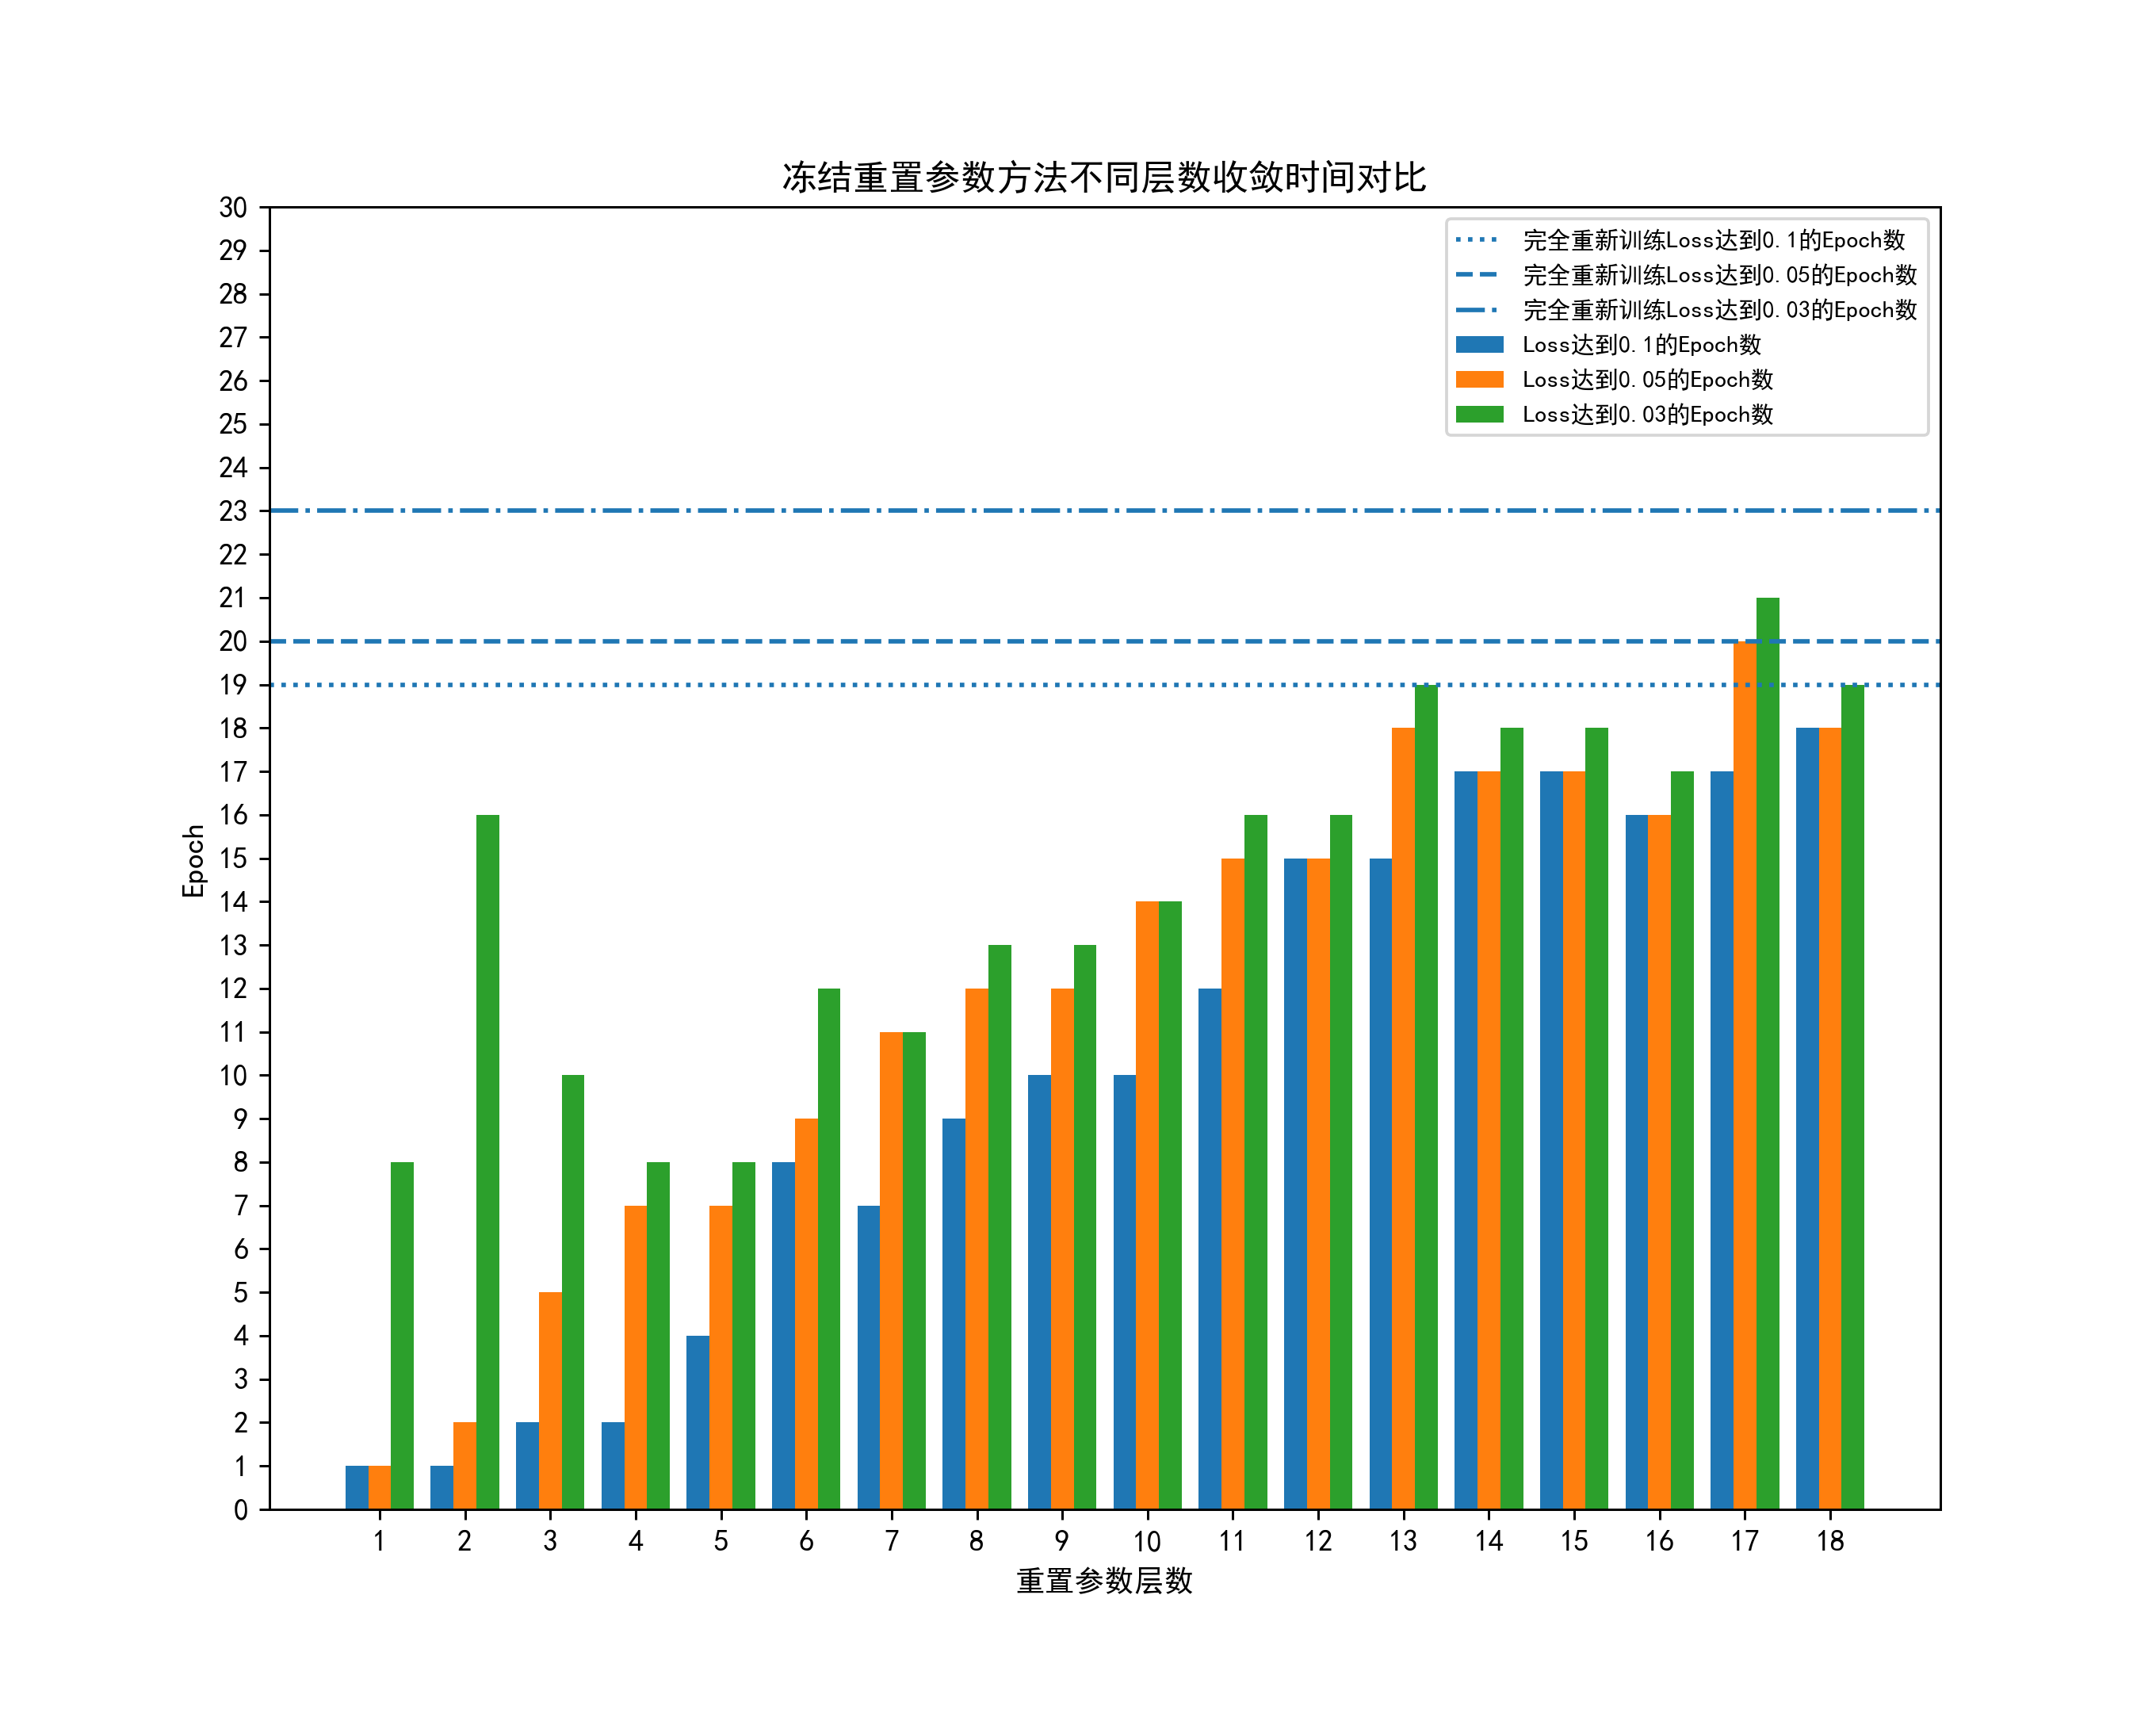
\includegraphics[width=1\linewidth]{chapter4_time_1.png}
    \caption{冻结重置参数方法不同层数收敛时间对比}
    \label{fig:chapter4_time_1}
\end{figure}
\\    如图\ref{fig:chapter4_time_1}所示,图中展示了本文所讲述的重置冻结参数遗忘方法在重置不同层次参数上使用保留集训练后收敛时间的对比。
图中展示了三套柱状对比图,蓝色柱图、黄色柱图和绿色柱图分别代表使用保留训练集训练网络时,该训练批次(Epoch)的平均损失函数loss的值首次降到0.1,0.05和0.03以下时的训练批次(Epoch)数。
批次数越小,说明训练的收敛时间越快。上面有三条不同线型的横线,分别代表为了遗忘一定的类别完全重新训练网络,该训练过程的平均损失函数值首次降到0.1,0.05和0.03以下时的训练批次(Epoch)数。
这三条横线的作用时与本文提到的方法进行收敛时间上的对比。
从图中的柱状图中可以看出,随着重置参数的层数逐渐增多,其收敛的Epoch逐渐增大,逐渐接近完全重新训练时收敛的Epoch。
其实这也不难理解,随着重置参数的层数增多,网络中需要更新的参数也逐渐增多,其状态也越来越接近完全重新训练的情况,所以收敛时间也逐步接近完全重新训练。
我们希望选择的层次是选择该层次后,训练后的准确率越高越好,训练收敛时间越快越好。
所以综合图\ref{fig:chapter4_1}和\ref{fig:chapter4_distance_1},可以备选的层次是前7层均在可以接受的范围内,重置参数层数越小,准确率越高,收敛时间也越快。
\begin{figure}
    \centering
    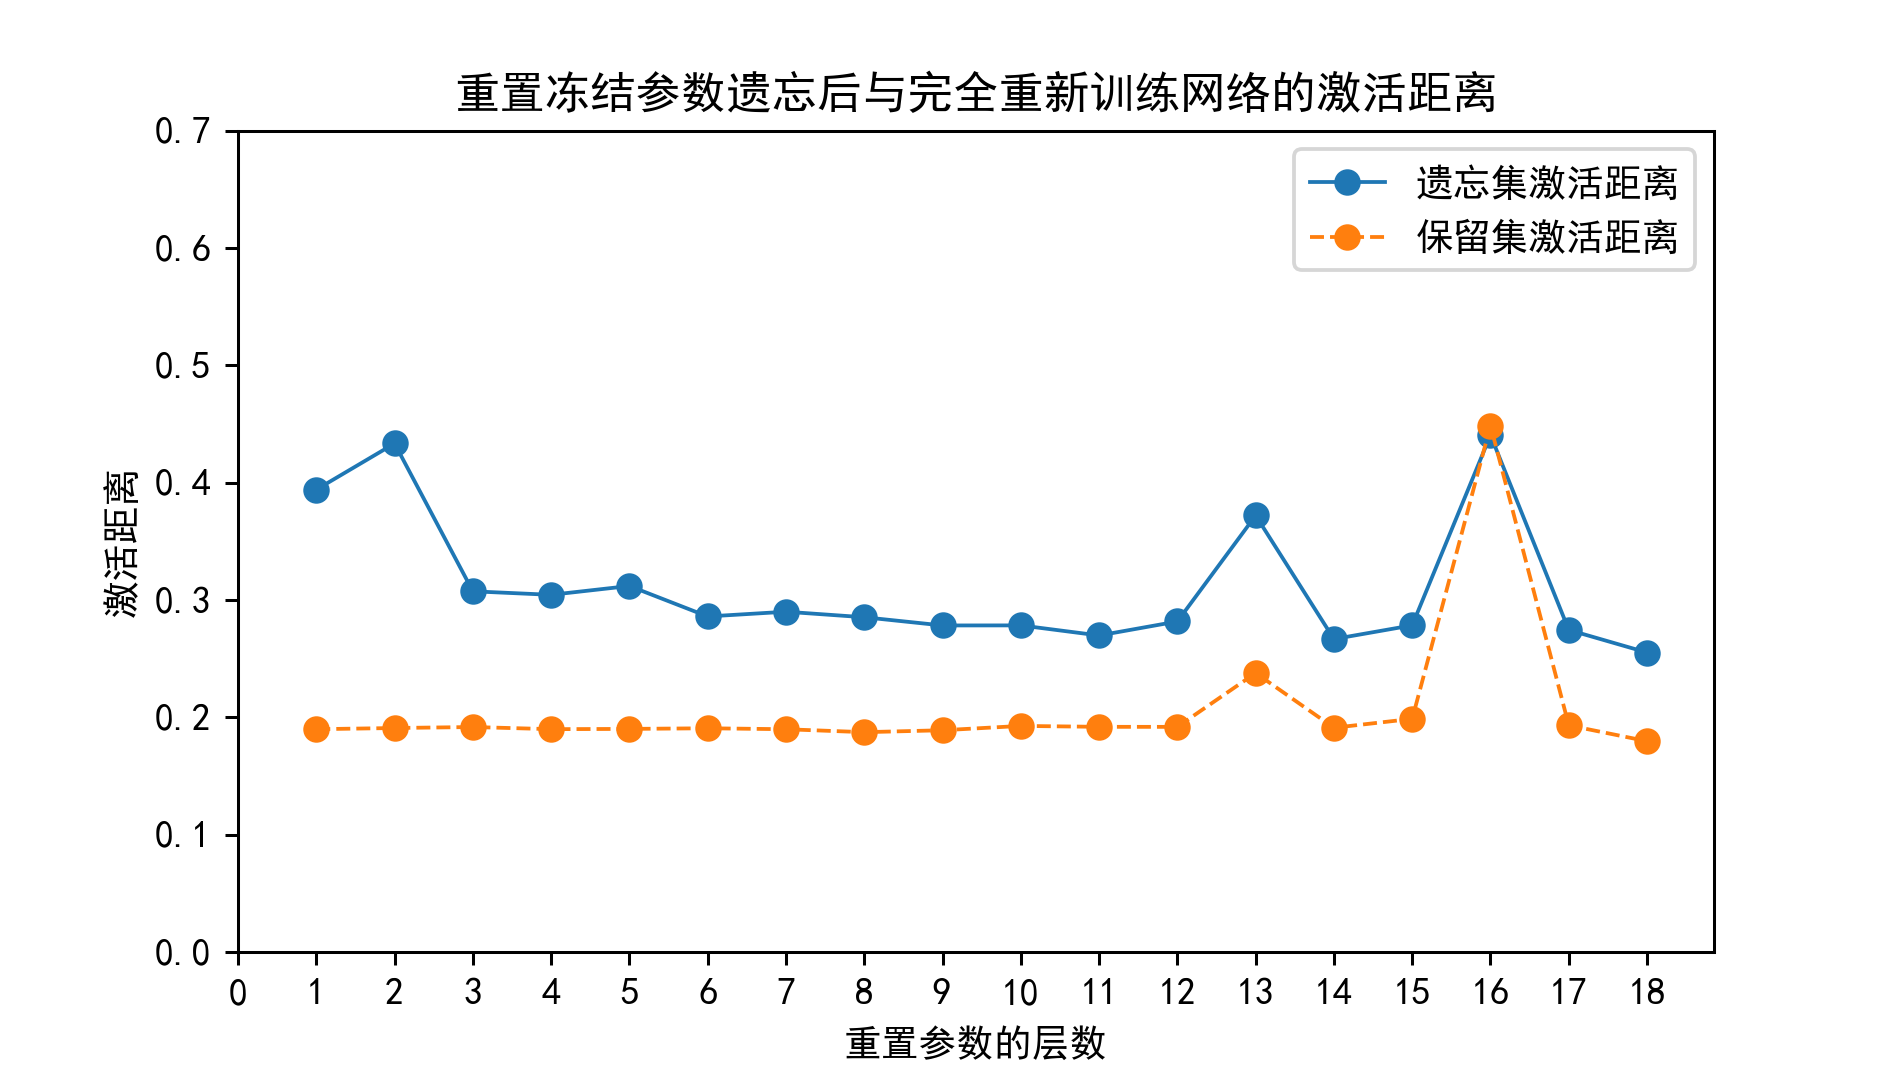
\includegraphics[width=0.9\linewidth]{chapter4_distance_1.png}
    \caption{重置冻结参数遗忘后与完全重新训练网络的激活距离}
    \label{fig:chapter4_distance_1}
\end{figure}
\\    如图\ref{fig:chapter4_time_1}所示,图中展示了本文所讲述的重置冻结参数遗忘方法训练的网络与完全重新训练所训练的网络之间对于测试集输出之间的距离差。
这个距离差在上一节有具体讲到,是两个网络输出向量差的绝对值的第二范数值。我们用这个范数值在测试数据集上的期望来作为两个网络的激活距离。
蓝色折线代表两个网络在遗忘集上的激活距离,橙色折线代表两个网络在保留集上的激活距离。从图中可以看出,两个网络在遗忘集上的激活距离要高于在保留集上的激活距离。
我们对于两个网络激活距离的期望是越小越好,在前7层可以看到保留集的激活距离普遍稳定地保持较低数值,而对于遗忘集的激活距离前2层的数值相对较大,3、4、5层数值也略大,从第6层开始,数值变得平稳。
因此,综合图\ref{fig:chapter4_1}和图\ref{fig:chapter4_time_1}和图\ref{fig:chapter4_distance_1}的分析结果,我们选择第6层作为重置冻结参数遗忘方法对于ResNet18网络重置参数的层数。
\subsection{冻结必要性验证实验}
\begin{figure}
    \centering
    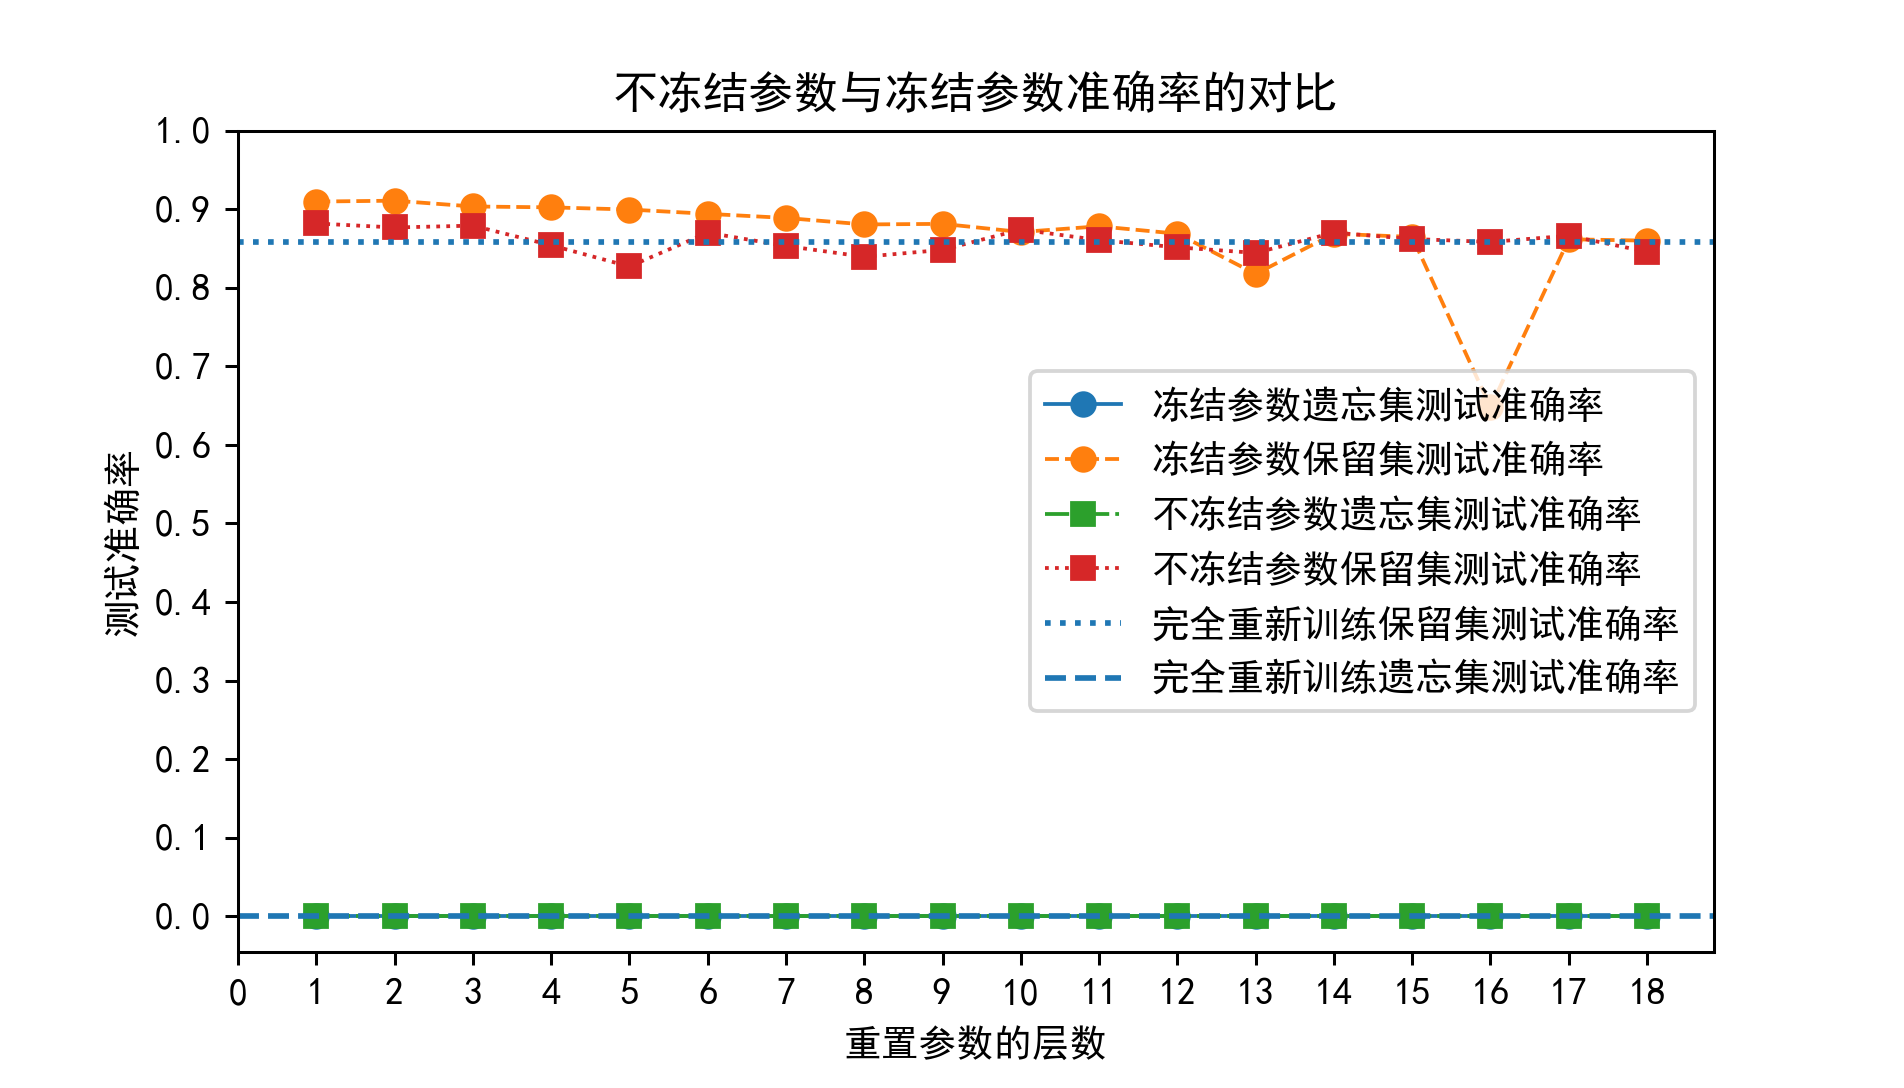
\includegraphics[width=0.9\linewidth]{chapter4_2.png}
    \caption{不冻结参数与冻结参数准确率的对比}
    \label{fig:chapter4_2}
\end{figure}
如图\ref{fig:chapter4_2}所示,图中展示了重置一定参数后冻结参数与不冻结参数训练对遗忘类别和保留类别准确率的影响。
橘黄色圆点折线代表冻结参数后使用保留训练集训练网络得到的网络在保留测试集上得到的准确率,蓝色圆点折线代表该网络的在遗忘测试集上得到的测试准确率。
红色方格折线代表不冻结参数的情况下使用保留训练集训练得到的网络在保留测试集上得到的测试准确率,绿色方格折线代表该网络在遗忘测试集上得到的测试准确率。
除此之外,图中还画了两条横线,圆点线代表完全重新训练的网络模型在保留测试集上得到的测试准确率,条状线段线代表完全重新训练的网络模型在遗忘测试集上得到的测试准确率。
这两条横线的主要作用是作为冻结参数和不冻结参数准确率的参照。通过橘黄色圆点折线和红色方格折线可以看出冻结参数与不冻结参数在保留集测试准确率上总体相差不大,但是冻结参数的方法要略好于不冻结参数方法。
在遗忘集的测试准确率上,两种方法效果相同,均为0。
\begin{figure}
    \centering
    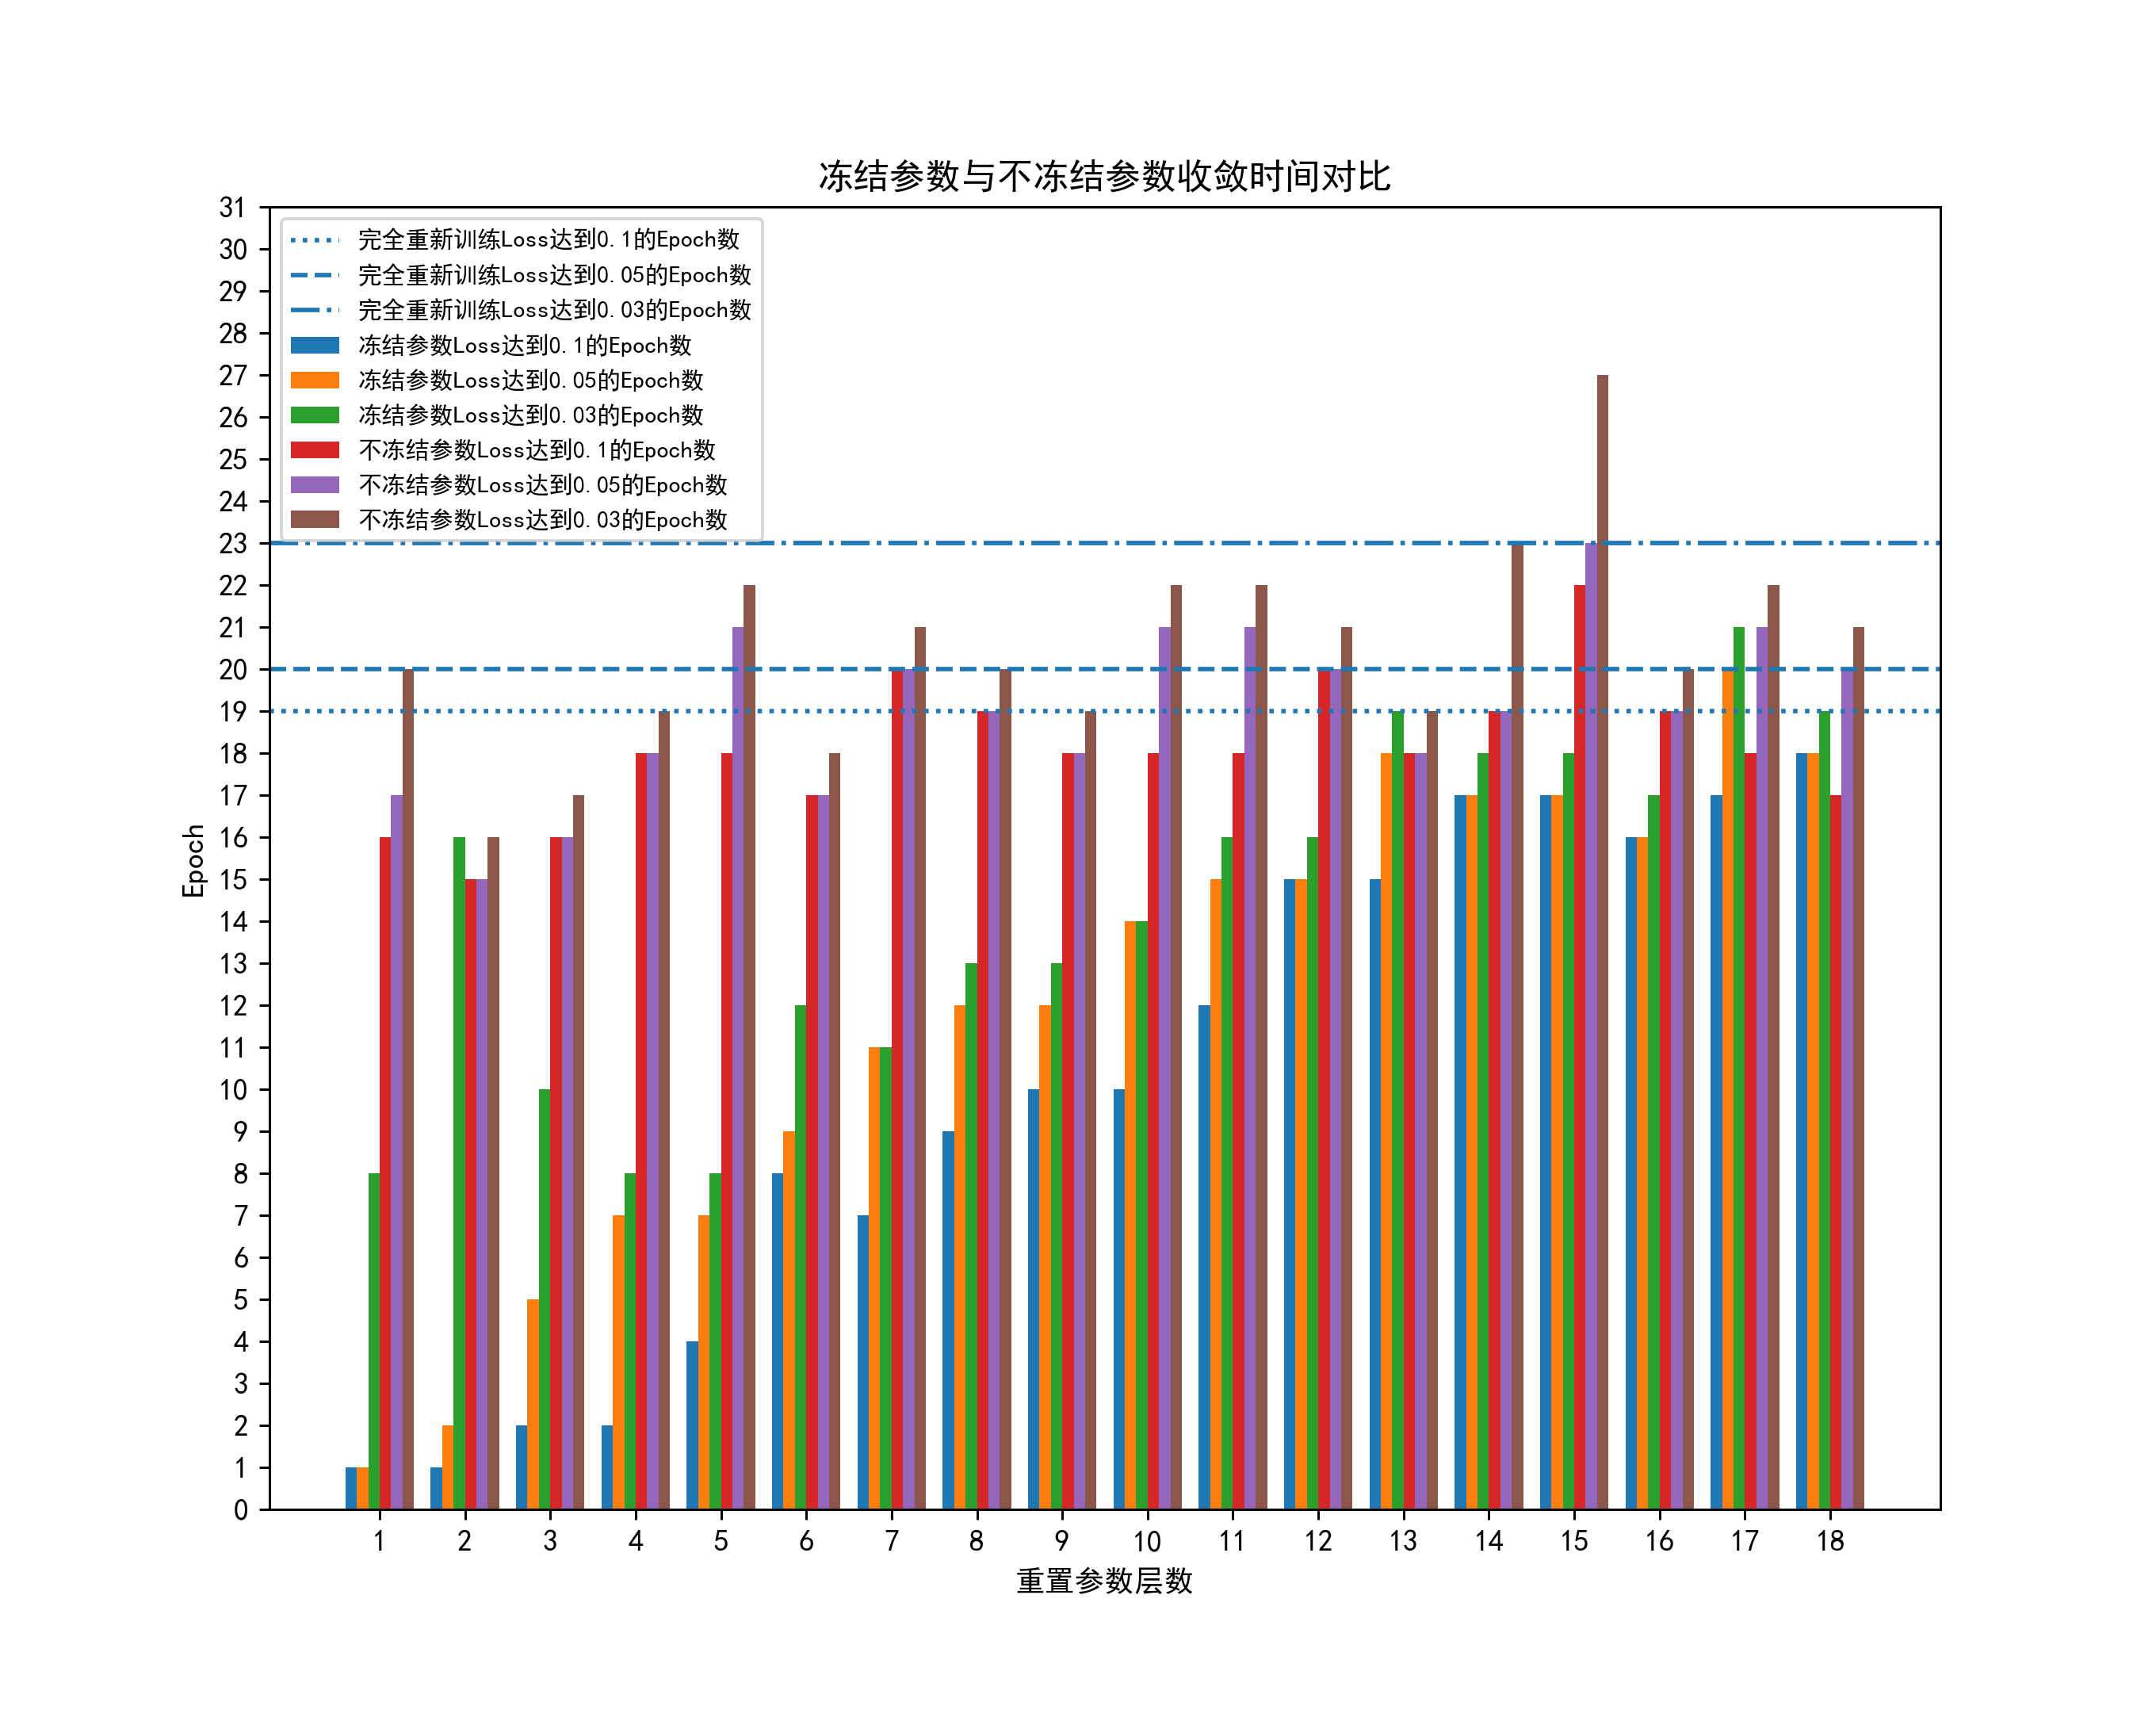
\includegraphics[width=1\linewidth]{chapter4_time_2.png}
    \caption{冻结参数与不冻结参数收敛时间对比}
    \label{fig:chapter4_time_2}
\end{figure}
\\如图\ref{fig:chapter4_time_2}所示,图中展示了冻结参数与不冻结参数重置参数后使用保留训练集训练网络的收敛时间。这个收敛时间同实验一的收敛时间定义相同。
蓝色、黄色和绿色柱图分别代表冻结参数情况下网络的平均损失函数值收敛到0.1、0.05和0.03时所花费的训练周期,即Epoch数。
粉色、紫色和棕色柱图分别代表非冻结参数情况下网络的平均损失函数收敛到0.1、0.05和0.03时所花费的训练周期数。
上面画出的三条横线,圆点线、条状线和点段线分别代表完全重新训练网络过程中,网络的平均损失函数值收敛至0.1、0.05和0.03时所花费的训练周期数。其主要作用是用来提供参照。
通过观察冻结参数和不冻结参数的柱状图可以发现,冻结参数后训练的收敛时间从整体上要少于不冻结参数训练网络收敛时间。这个现象也是符合分析的逻辑,冻结参数后,一部分参数不需要计算更新,而没有冻结参数的网络则需要计算所有参数的更新,从计算量上分析,不冻结参数训练网络所需要的工作量是比冻结参数要大的。
通过图\ref{fig:chapter4_2}和图\ref{fig:chapter4_time_2}的分析结果可以初步得出结论,冻结参数训练网络的方法要好于不冻结参数训练网络的方法。
\begin{figure}
    \centering
    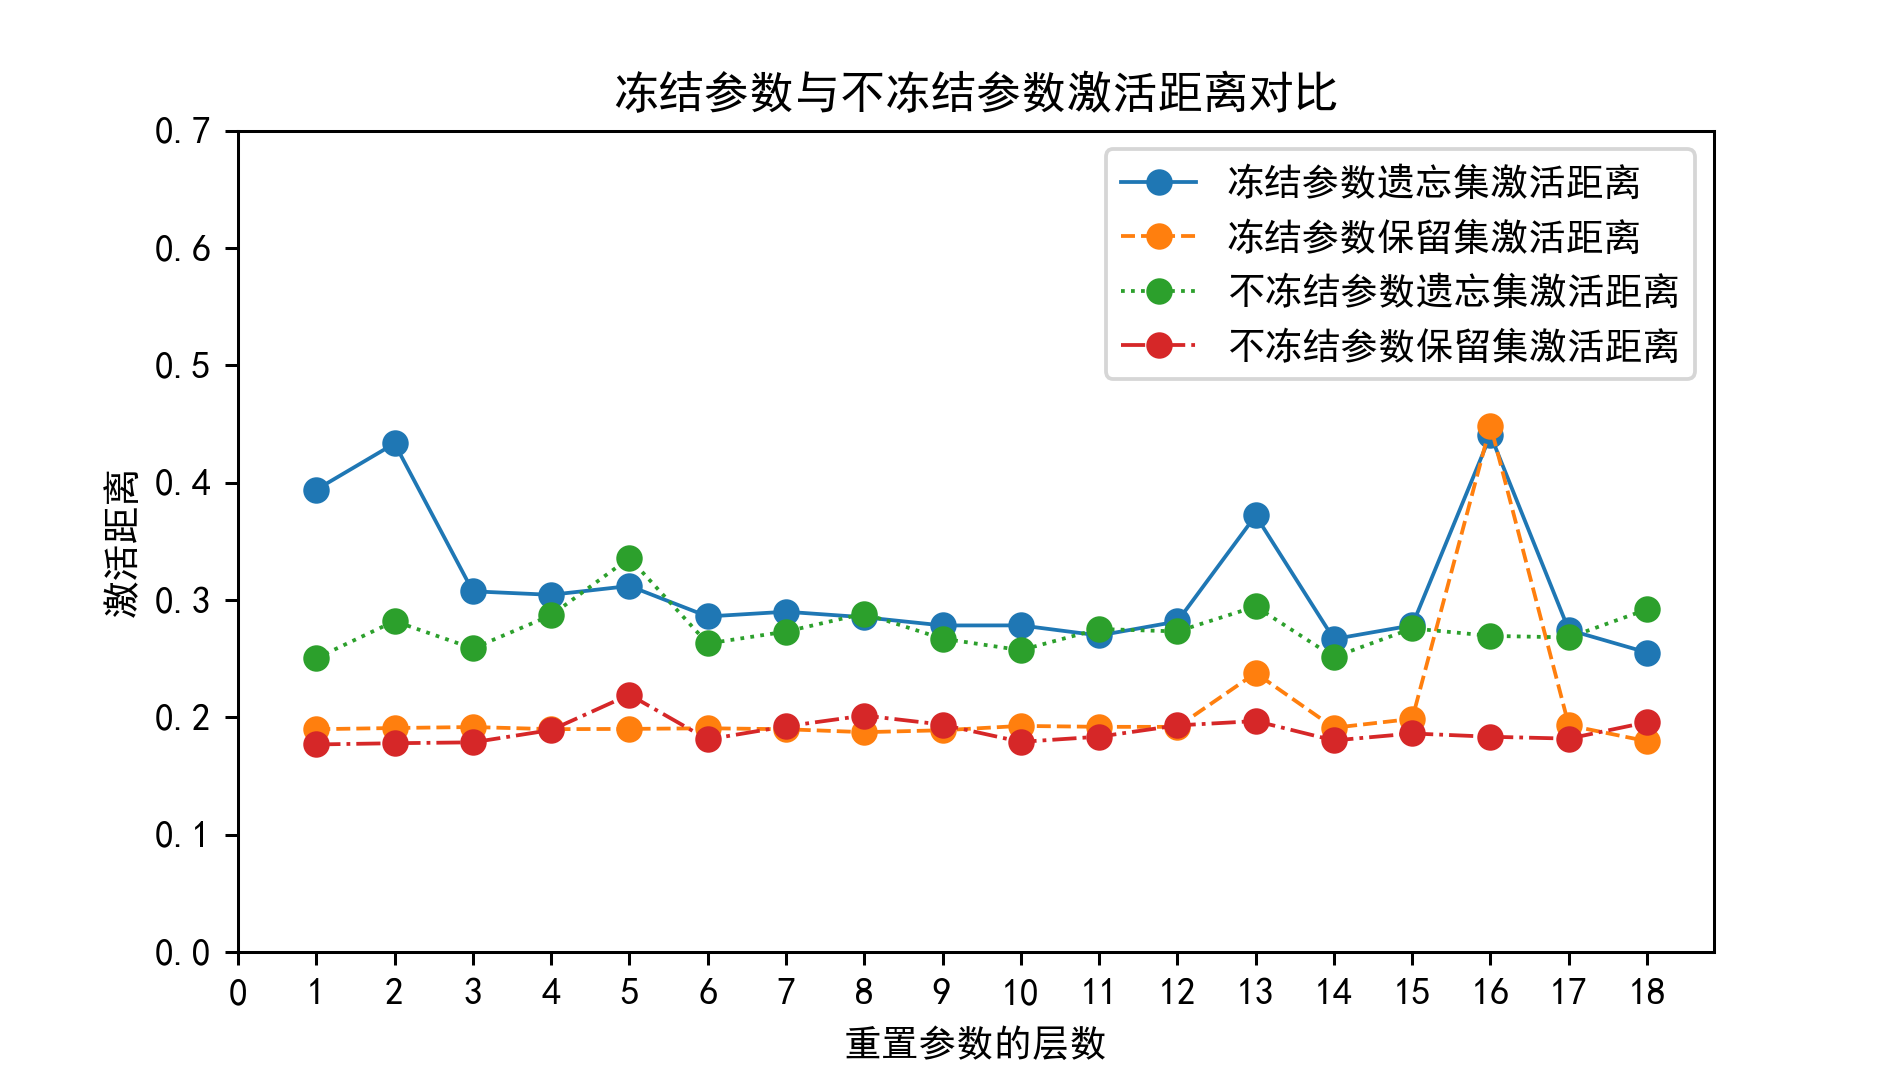
\includegraphics[width=0.9\linewidth]{chapter4_distance_2.png}
    \caption{冻结参数与没冻结参数激活距离对比}
    \label{fig:chapter4_distance_2}
\end{figure}
\subsection{反向冻结验证实验}
\begin{figure}
    \centering
    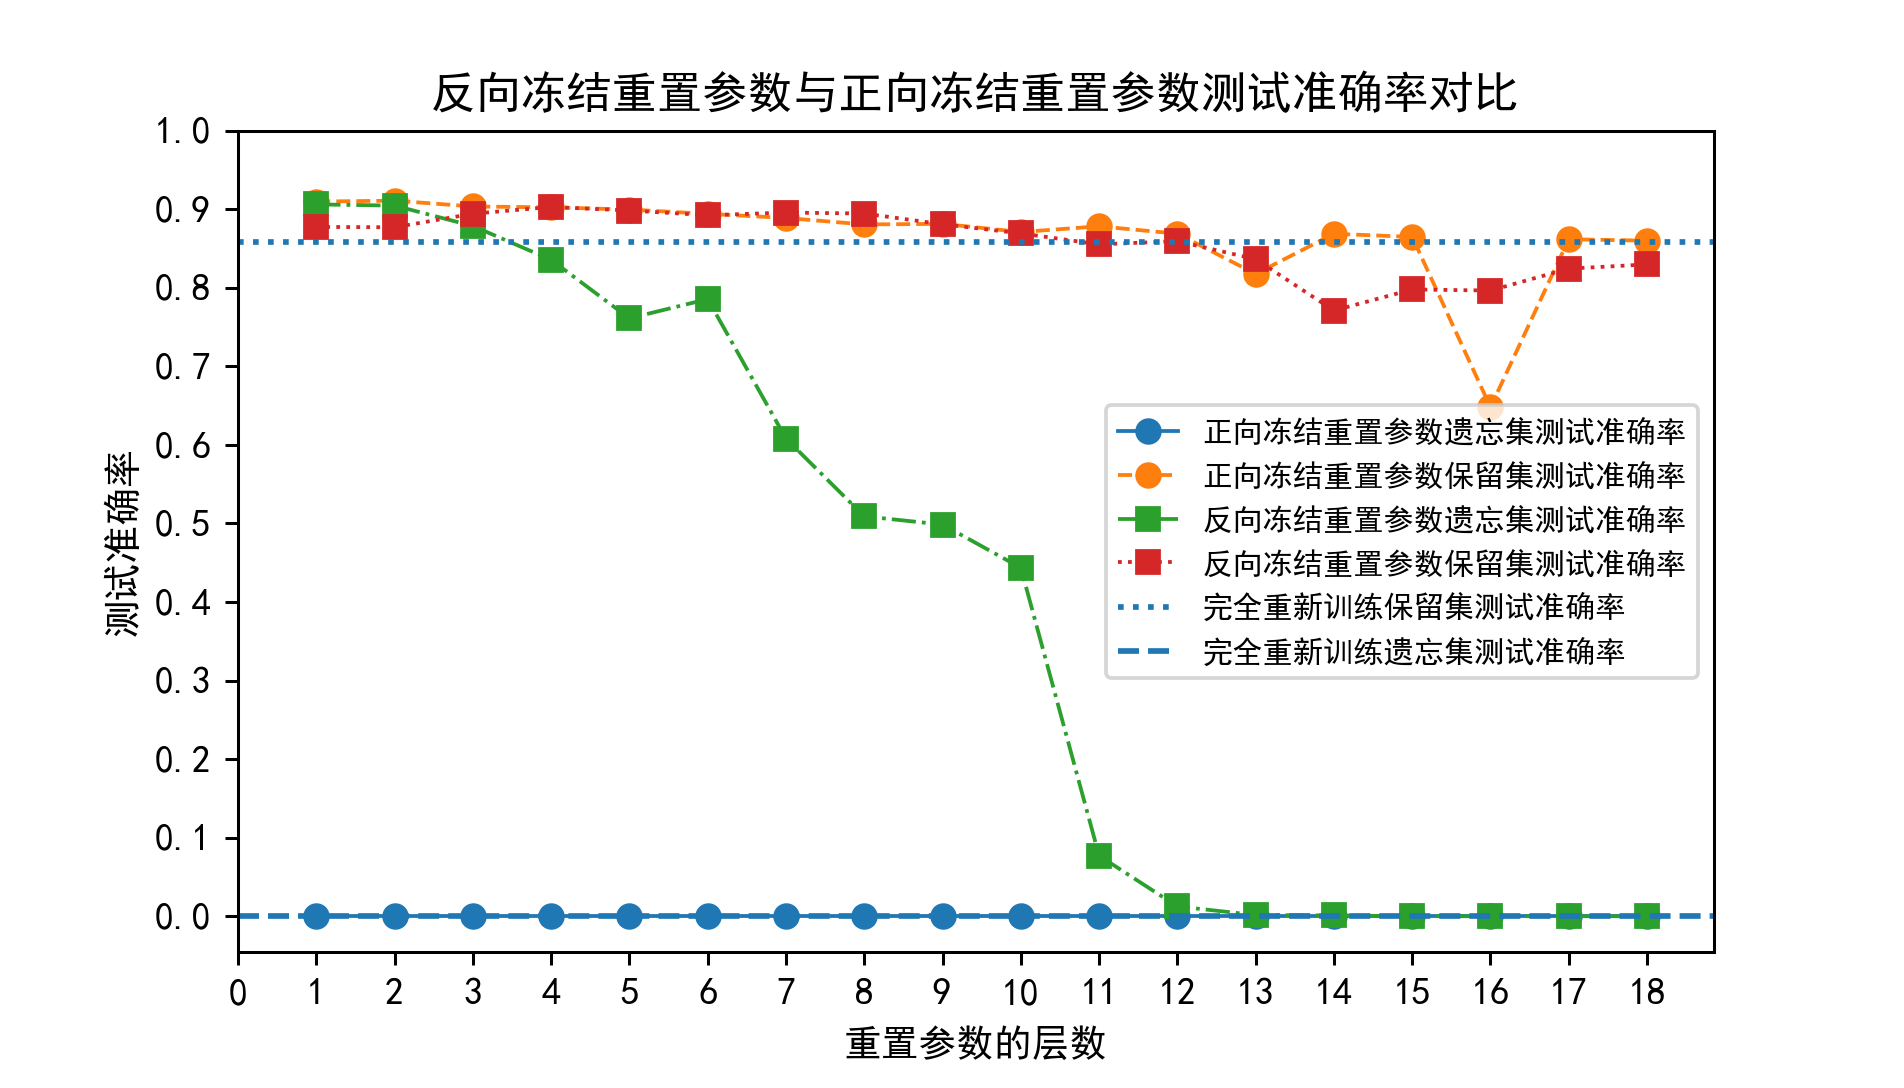
\includegraphics[width=0.9\linewidth]{chapter4_3.png}
    \caption{反向冻结重置参数与正向冻结重置参数测试准确率对比}
    \label{fig:chapter4_3}
\end{figure}
\begin{figure}
    \centering
    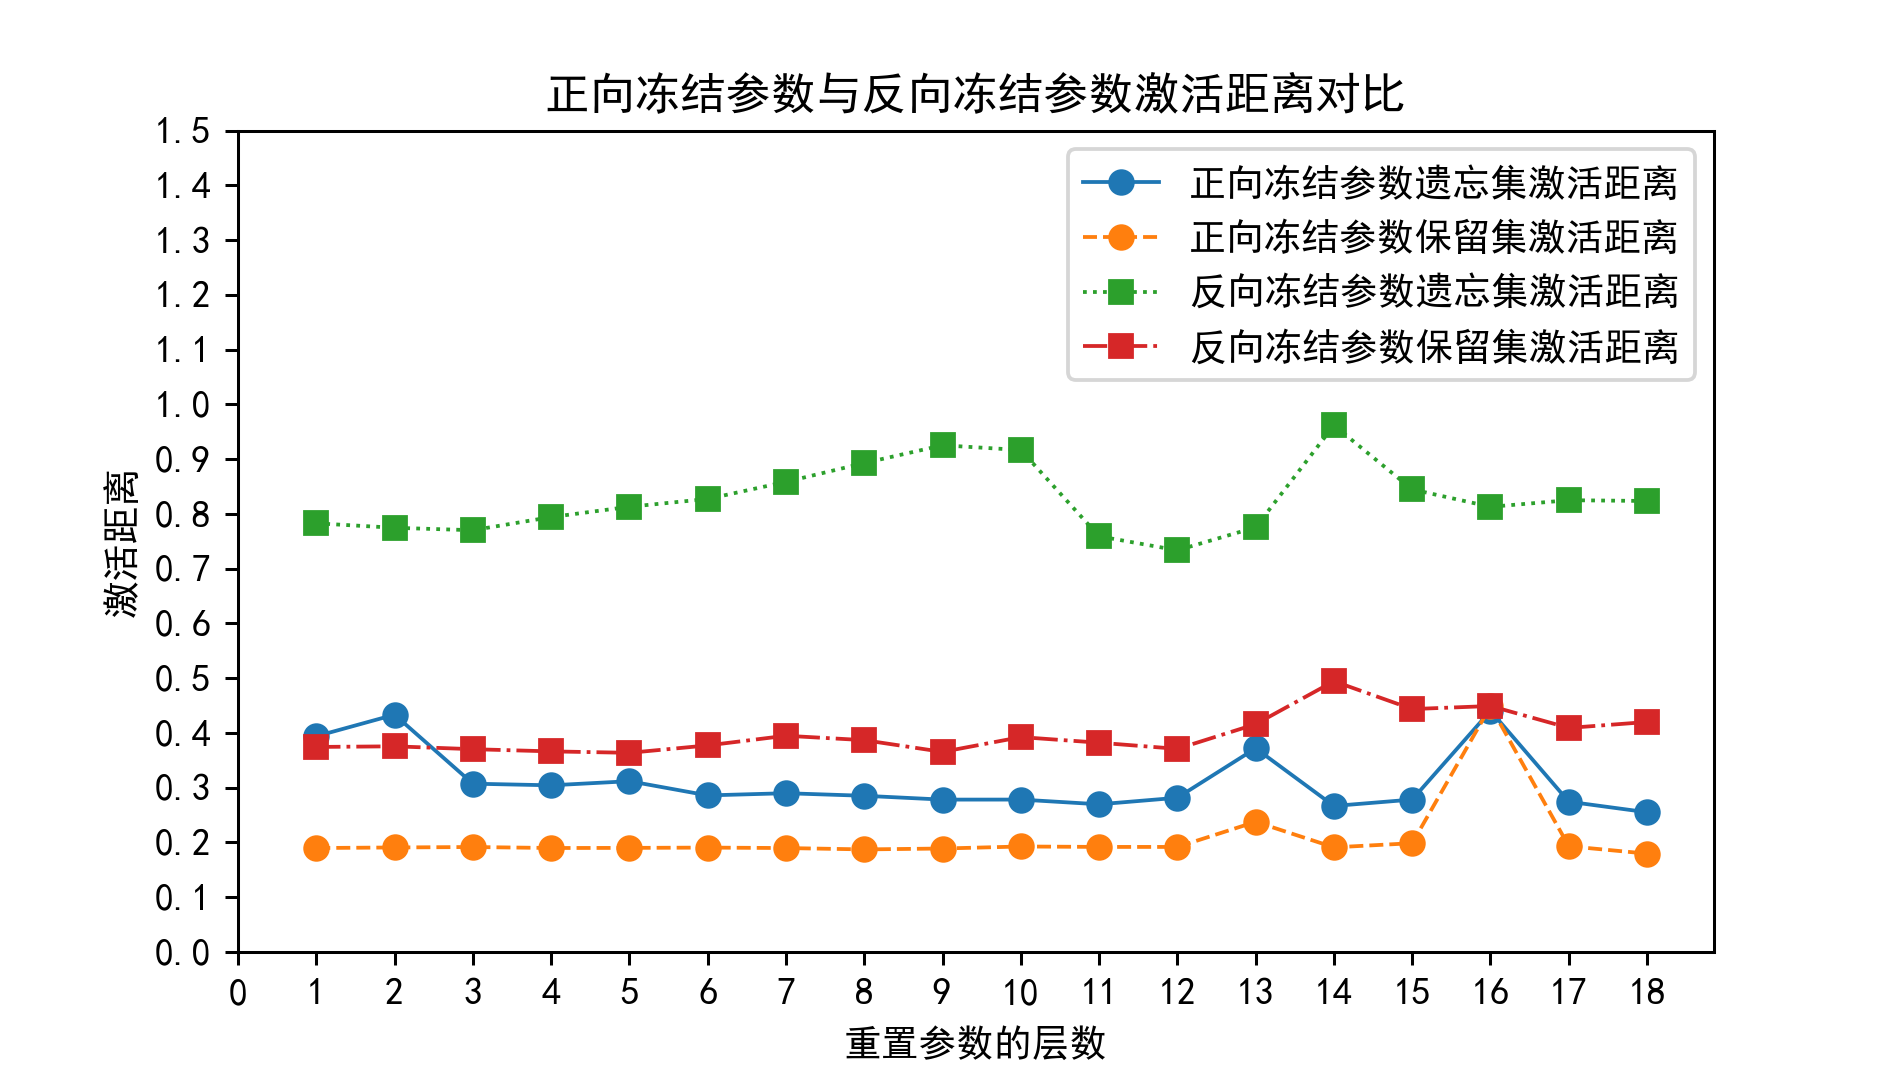
\includegraphics[width=0.9\linewidth]{chapter4_distance_3.png}
    \caption{正向冻结参数与反向冻结参数激活距离对比}
    \label{fig:chapter4_distance_3}
\end{figure}
\subsection{遗忘可持续性验证实验}
\begin{figure}
    \centering
    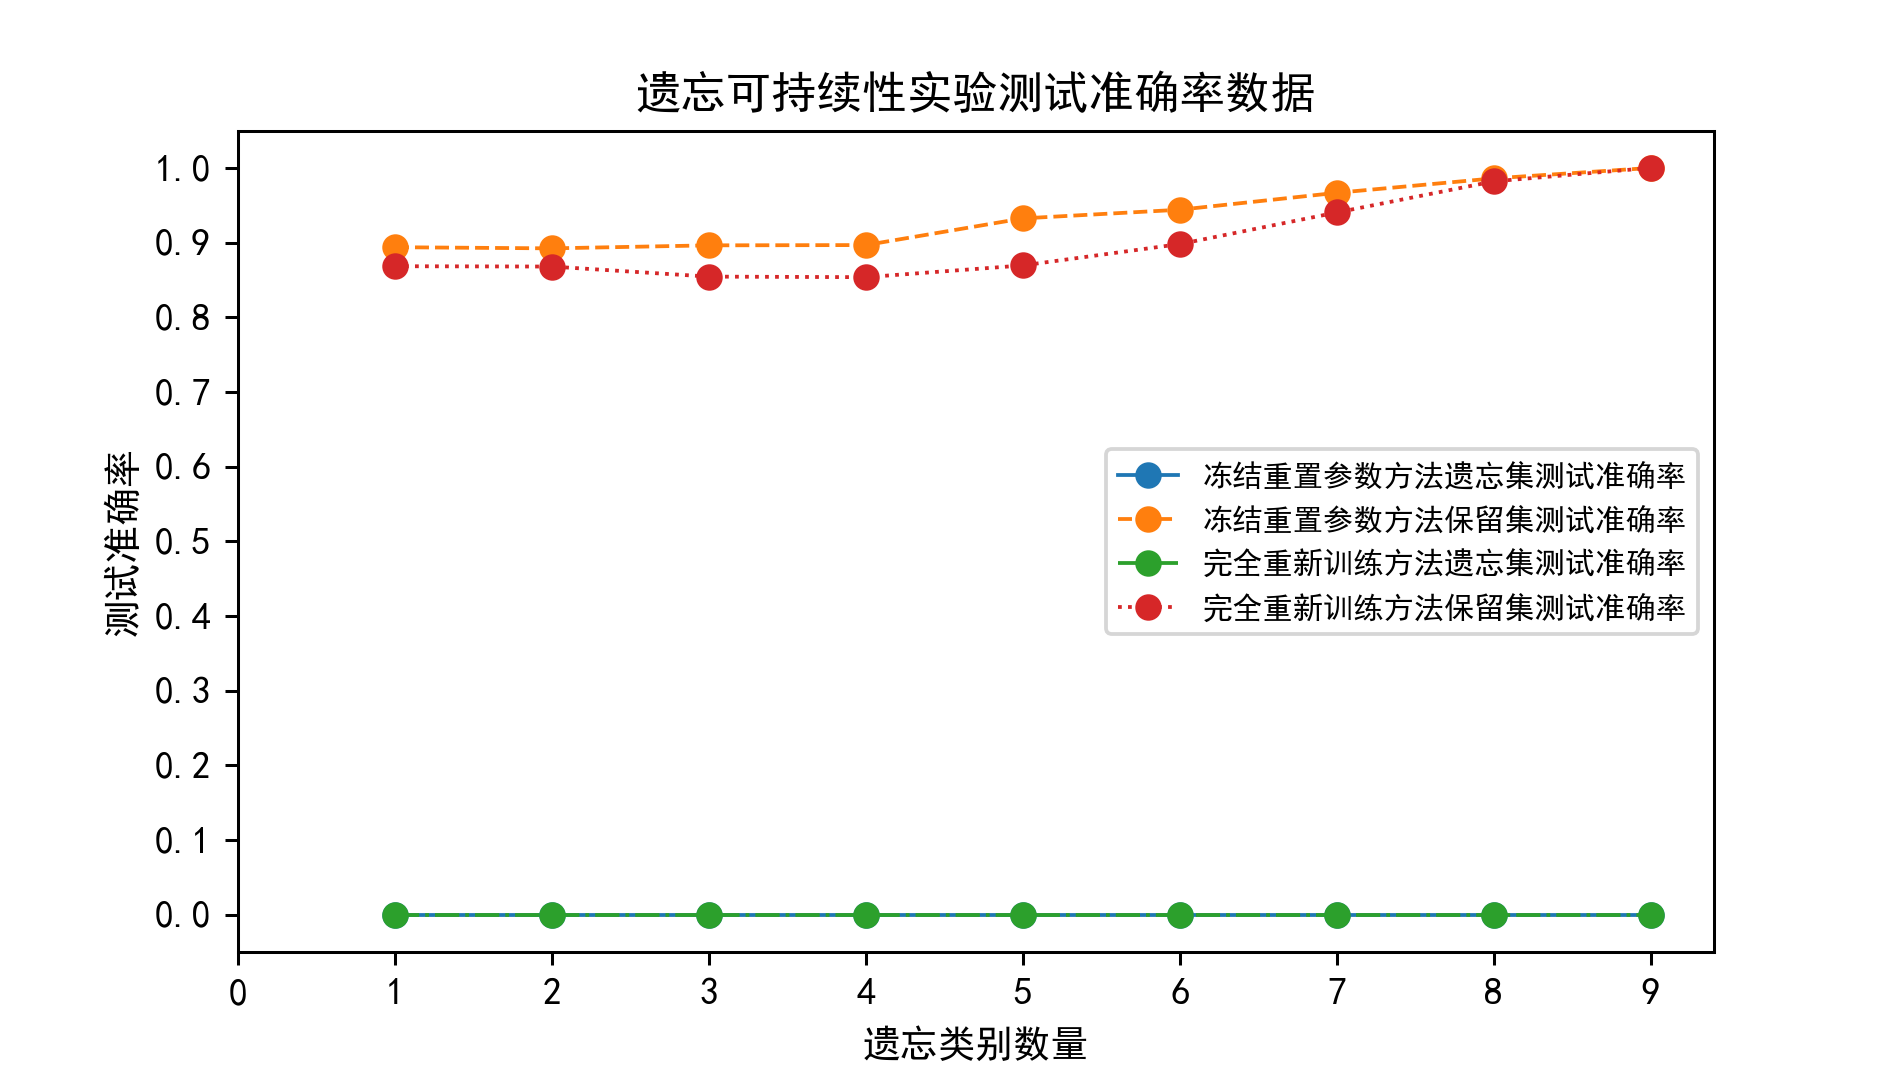
\includegraphics[width=0.9\linewidth]{chapter4_4.png}
    \caption{遗忘可持续性实验测试准确率数据}
    \label{fig:chapter4_4}
\end{figure}
\begin{figure}
    \centering
    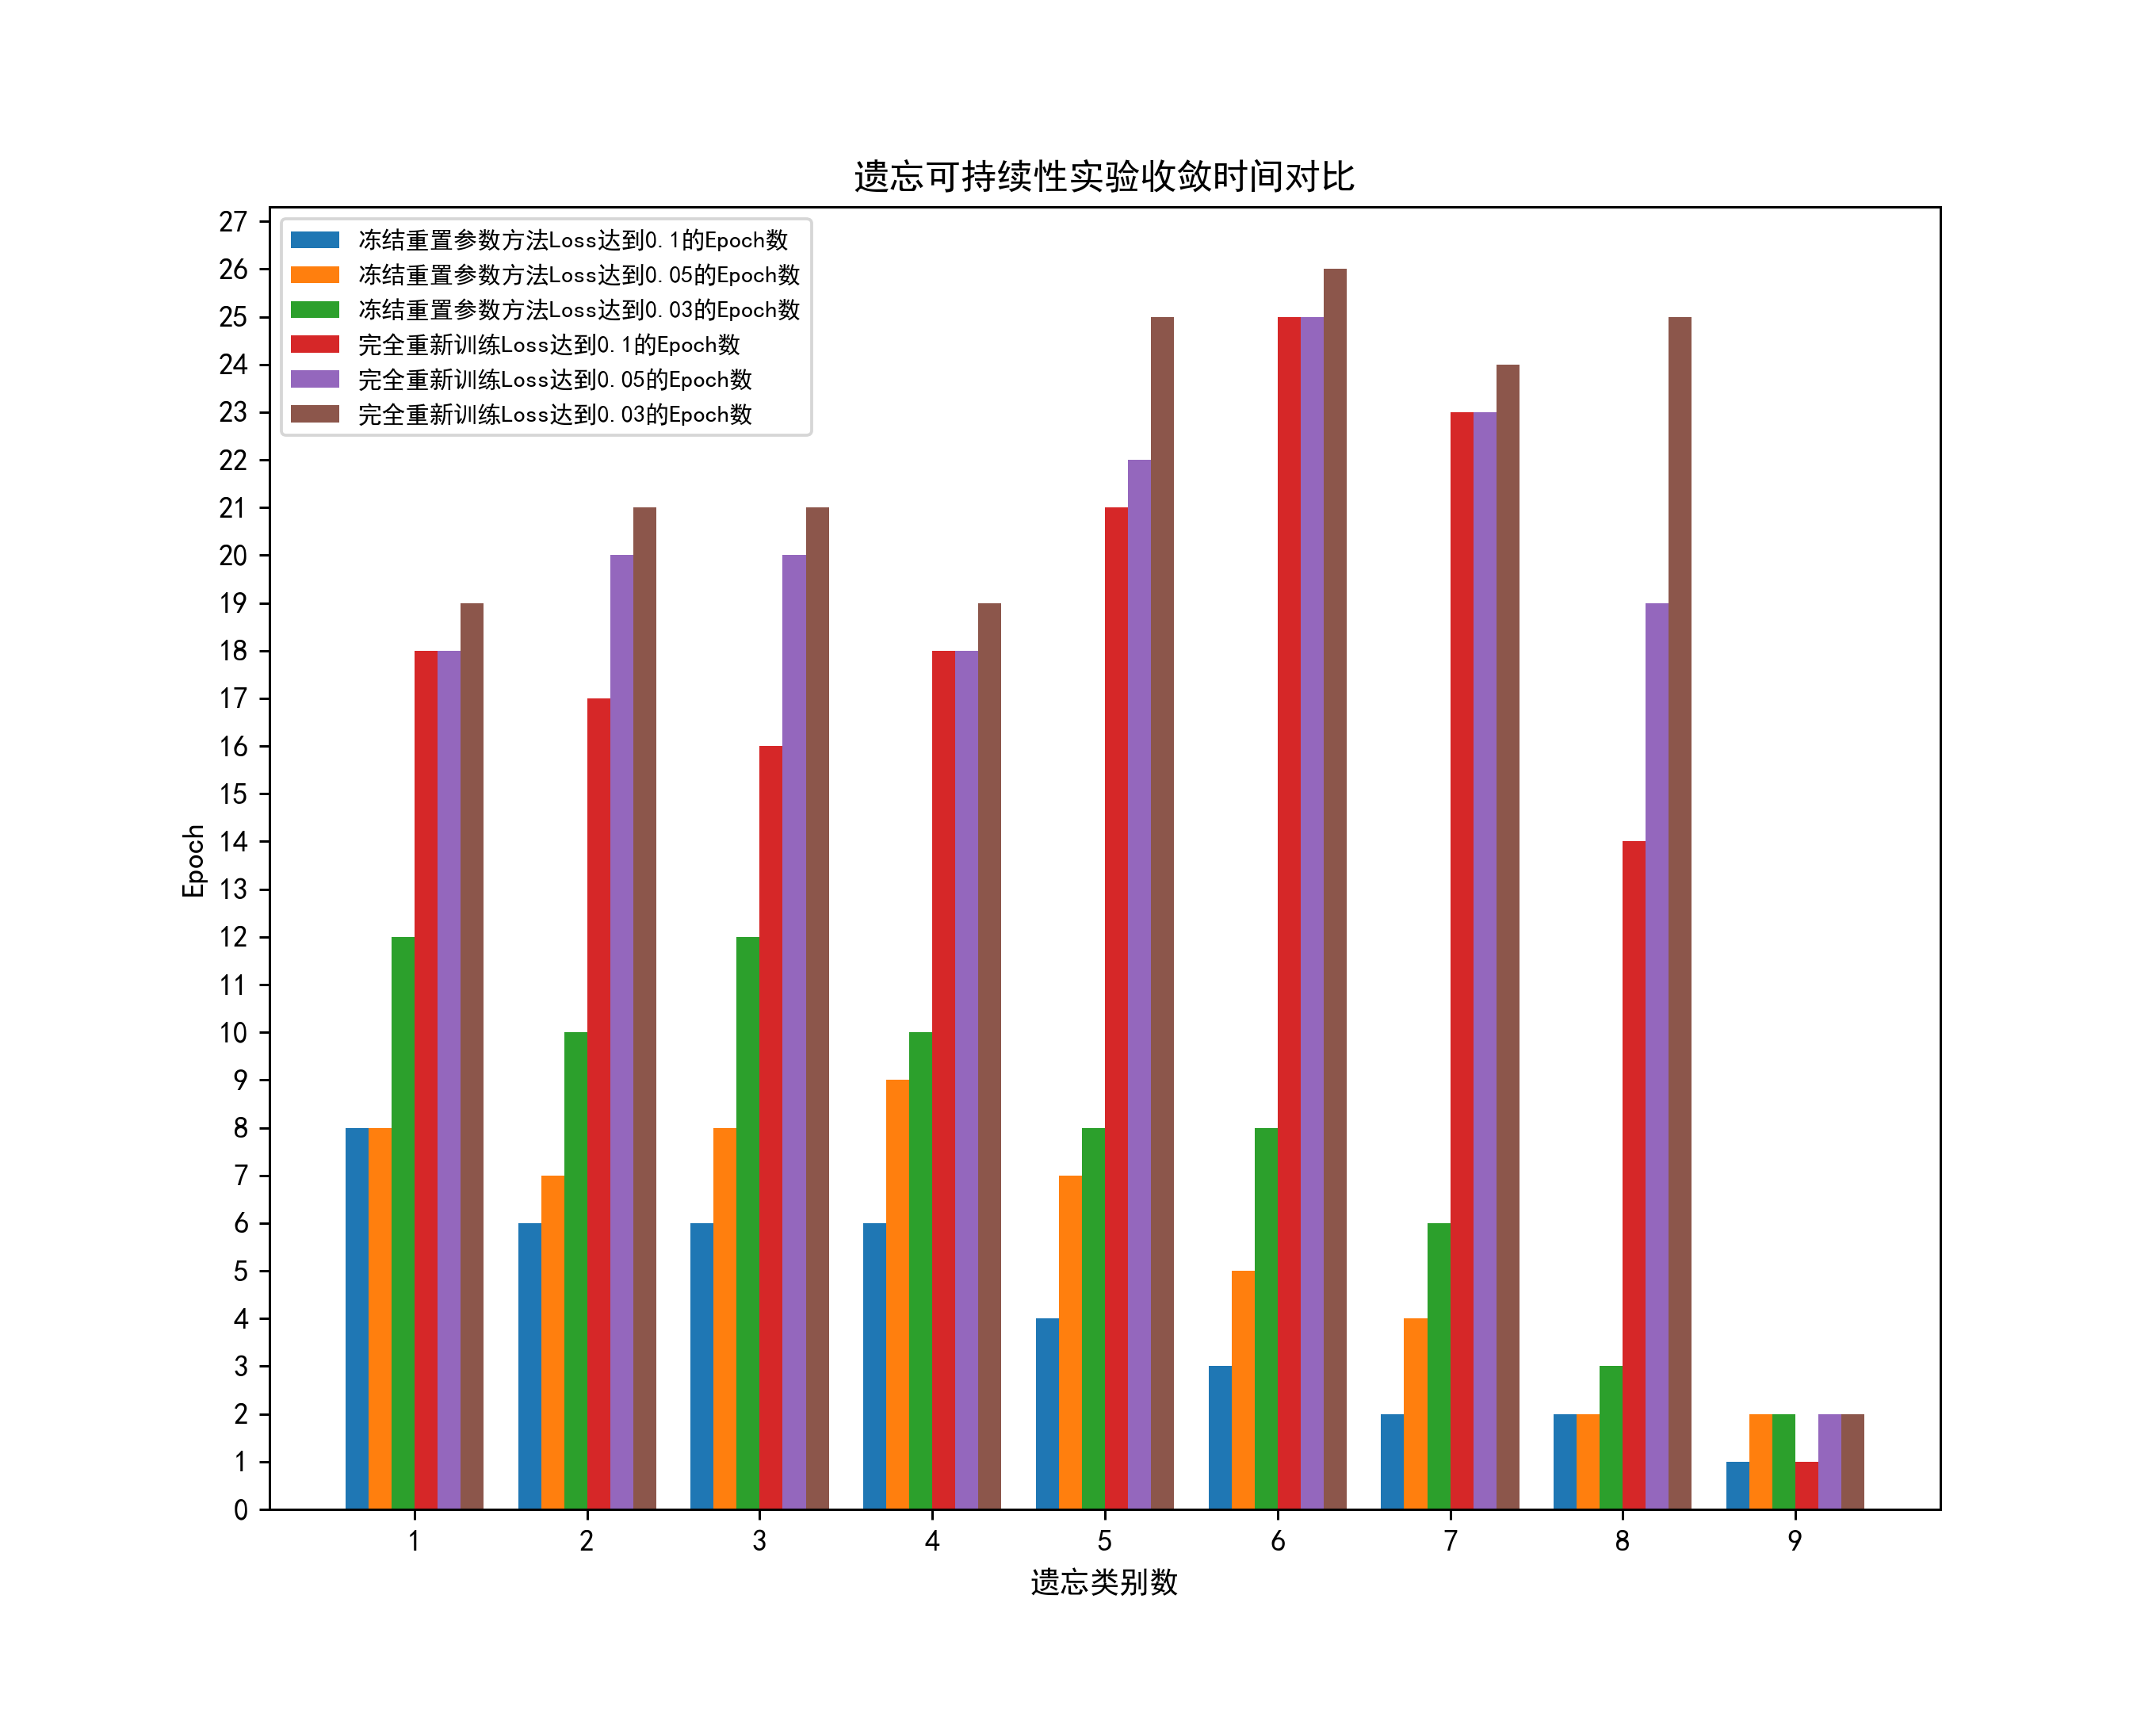
\includegraphics[width=1\linewidth]{chapter4_time_3.png}
    \caption{遗忘可持续性实验收敛时间对比}
    \label{fig:chapter4_time_3}
\end{figure}
\begin{figure}
    \centering
    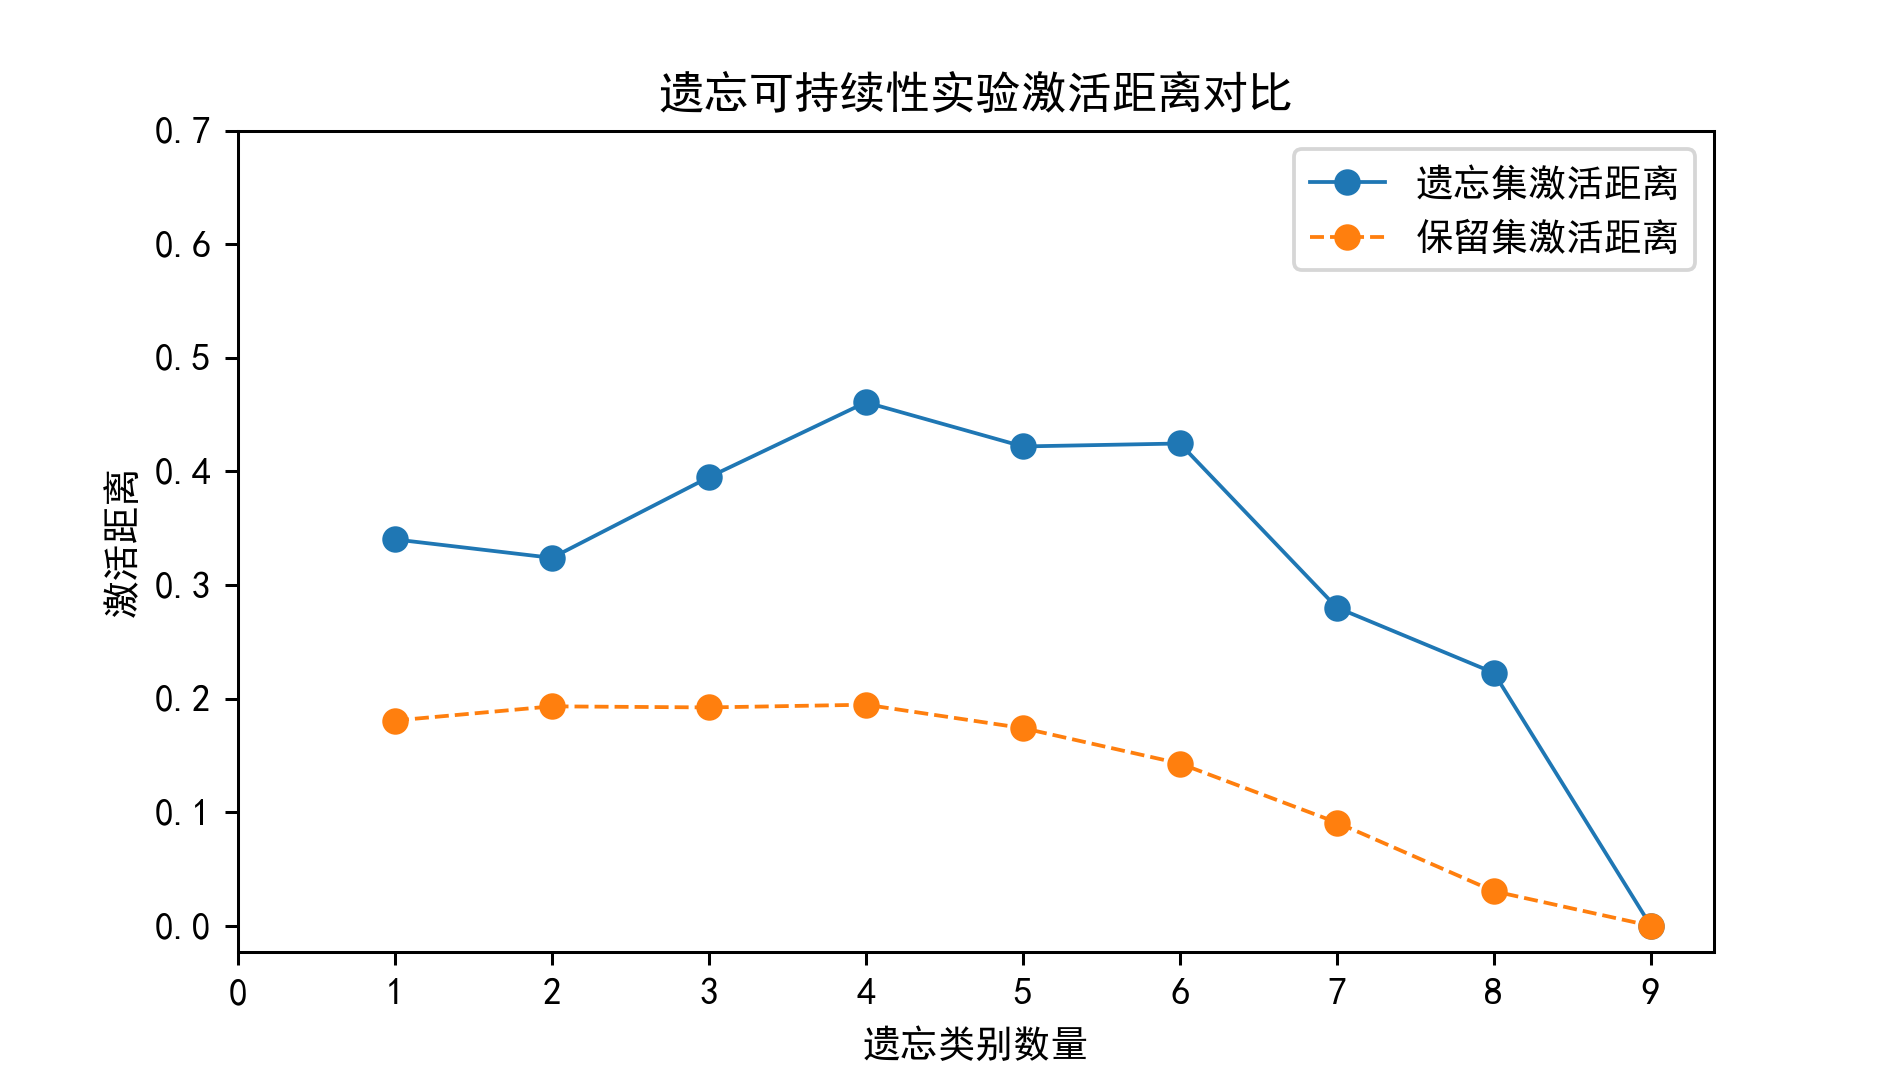
\includegraphics[width=0.9\linewidth]{chapter4_distance_4.png}
    \caption{遗忘可持续性实验激活距离对比}
    \label{fig:chapter4_distance_4}
\end{figure}
\section{本章小结}


%% !TeX root = ../thuthesis-example.tex

\chapter{总结与展望}

\section{研究工作总结}

本文通过理论假设和实验验证的方法针对卷积神经网络如何遗忘的问题进行了系统研究。本文正文共有五个章节,分别是引言、相关研究工作、卷积神经网络的分层抽象特性与遗忘方法、遗忘方法的实现和验证以及总结和展望。

第一章引言中首先介绍了遗忘问题产生的背景与研究的意义。随着卷积神经网络的广泛应用,越来越多的数据被用于卷积神经网络的训练中。然而,随着在线机器学习服务的兴起,带来的问题愈加明显。
有一些研究者发现通过仅仅通过神经网络的输出数据就能对神经网络模型的输入数据进行还原,或者对神经网络模型训练出来的参数进行抽取,或者能判断出某个输入是否曾经被用于训练该模型。
这些攻击手段的出现给我们发出的一个明显信号就是神经网络模型中包含重要的信息,很可能会出现数据泄露甚至个人隐私数据泄漏的问题。这是从实际出发提出来的数据需要遗忘的需求。
从法律角度上看,机器学习模型也是需要遗忘的。欧盟出台的《通用数据保护条例(GDPR)》从法律层面上规定了用户拥有“被遗忘权”。当用户需要删除数据时,数据管理者要及时履行约定。
基于这些事实,我们研究卷积神经网络的遗忘具有重要的现实意义。
接着,第一章介绍了卷积神经网络遗忘技术的最新发展现状。经过搜集和整理后发现,目前针对卷积神经网络的遗忘问题研究者们提出了多种解决方案,例如基于牛顿梯度更新的方法和基于网络分割的方法等,但是还没有一个成熟稳定的理论。
随后,第一章介绍了本文设计遗忘方法的主要思想和实验验证的效果。在第一章最后介绍了本文主要的写作框架。

在第二章中,本文主要介绍了和卷积神经网络研究方向相关的具有代表性的研究工作,具体的方向涉及到迁移学习,增量学习还有遗忘学习。
迁移学习的思想和本文的思路在某种程度上是契合的,目的都是无需重新训练整个模型就能将快速地实现模型知识的迁移,对本文具有一定的启发意义。
增量学习技术的出发点是克服神经网络本身固有的特点,即灾难性遗忘。随着新的训练数据继续在网络中训练,原先已经训练过的类别在准确率上有不同程度的降低,即发生了灾难性遗忘的现象。
为了解决这个问题,研究人员尝试了多种在无需重新训练全部模型的情况下,想办法将新的类别加入到原有的网络模型当中。其中有一类方法就是共享网络参数的方法,就是将低层次的网络参数作为共享参数,然后不断地在靠近输出的层次上面增加神经网络,同时冻结共享参数。
然而,这样的方法对于增量学习来说具有一定的挑战性。因为新类别的数据可能具有自己独特的基本特征,如果冻结较为低层次的网络参数,可能会导致无法学习新类别的这些基本特征信息。
但是对于神经网络的遗忘就无需考虑这个问题,因为类别是在减少的,不用担心会有新的基本特征需要学习。
在遗忘学习的研究方面,一些研究人员已经尝试使用牛顿更新的方法,试图将消除待遗忘的训练数据带来的影响,可是效果不是很理想。
另外一些相关工作试图使用差分隐私的思路,给网络中的参数增加噪音,从而达到遗忘的目的。然而这样的方法会给保留的类别带来准确率下降的问题。总之,在卷积神经网络的遗忘方面尚没有成熟的理论。

第三章是本文的核心章节,在第三章为了让读者更好地理解卷积神经网络的分层抽象特性,我们首先介绍了卷积神经网络基本结构和原理。
接着介绍了卷积神经网络的分层抽象特性。就是卷积神经网络在较低层次提取的是输入的一些基本信息,就好像人类视觉中的具有差异性的感受野,有的感受野对横向移动感兴趣,有的感受也对纵向移动感兴趣。
随着卷积网络层次的提高,卷积核中提取的特征越来越抽象,感受野也越来越大,从而提取到特征的范围也越来越大。靠近输出层的卷积层提取到的是和分类相关的特征。
从这个特性我们受到了一定的启发,能不能不用更新所有的网络参数,只更新和分类关联比较大的网络参数。带着这个思路我们设计了一套遗忘方法,首先确定分层的数值。
为了确定这个数值,我们综合考虑了三个指标的数值。确定好分层后,接下来就要重置网络参数,我们首先将网络训练的初始参数保留下来,然后待需要重置参数时,将初始参数复制到相对应的层次上,这就完成了参数的重置过程。
再使用保留集对网络进行冻结部分参数的训练,被冻结的参数是没有被重置的参数,这么做是为了共享之前已经学习好的基本特征。
训练至网络收敛之后就完成了卷积神经网络的遗忘过程。我们为了测试遗忘的效果,选取了三个不同方面的测试指标,分别是测试集准确率,收敛时间还有激活距离。

第四章是对第三章遗忘方法的实验验证。我们设计了四个实验来进行验证,分别是确定冻结层数实验,冻结必要性验证实验,反向冻结验证实验和遗忘可持续性验证实验。确定冻结层数实验,目的是确定冻结参数的层次。
实验结果表明,对于Resnet18的网络结构来说,重置倒数第6层是个很好的选择。
冻结必要性实验的目的是对比更新网络参数后是否有必要对网络进行冻结。实验中设计了一套对比实验,通过三个指标的对比表明,冻结参数对提高遗忘效果是有必要的。
反向冻结实验作为本文提到的遗忘方法的一个对照实验,目的是验证分层抽象特性的有效性。从实验结果来看,分层抽象特性的效果是很明显的。
最后一个实验是遗忘可持续性验证实验,这个实验旨在探究本文提到的遗忘方法是否能够用来连续进行遗忘操作。最终实验结果表明,无论需要遗忘多少类别,本方法是均可以达到理想的遗忘效果。

\section{存在问题与展望}
随着卷积神经网络的应用越来越多,会有越来越多的数据被用来训练网络。GDPR法规的出台,神经网络不仅要研究如何训练,也要注意如何才能使得学习到的信息不能被攻击者窃取。
用户的隐私意识也在逐步地增强,相信会有越来越多的用户会提出要数据控制者删除数据的需求。本文虽然在一定的范围内取得了很好的效果,但是仍有以下几点不足。

第一,本方法只能针对保留数据集的情况下使用。有一些实际情况是训练数据不是实时可用,这就导致重置网络参数后无法恢复保留类别原有的准确率。如何不用保留数据集就能实现很好的遗忘效果是一个值得后续研究的方向。

第二,本方法只适用于遗忘整个类别的情况,对于遗忘单个数据的操作,本方法不能做到很好的支持。作者认为有一些数据一旦被用于学习以后,其影响是无法消除的,因此无法被遗忘,有一些相关工作\cite{2018arXiv181205159T}的结论也支持这一点。

\section{本章小结}
本章对全文进行了概括性的总结并对本文目前尚未做到的工作进行了说明,同时又进行了一定的展望。随着卷积神经网络的普遍应用,用户隐私越来越受到重视,基于卷积神经网络的遗忘方法的相关研究势在必行。
% !TeX root = ../thuthesis-example.tex

\chapter{图表示例}

\section{插图}

图片通常在 \env{figure} 环境中使用 \cs{includegraphics} 插入,如图~\ref{fig:example} 的源代码。
建议矢量图片使用 PDF 格式,比如数据可视化的绘图;
照片应使用 JPG 格式;
其他的栅格图应使用无损的 PNG 格式。
注意,LaTeX 不支持 TIFF 格式;EPS 格式已经过时。

\begin{figure}
  \centering
  \includegraphics[width=0.6\linewidth]{example-image-a.pdf}
  \caption{示例图片}
  \label{fig:example}
\end{figure}

若图或表中有附注,采用英文小写字母顺序编号,附注写在图或表的下方。
% LaTeX 传统上一般将附注的内容同图表的标题写在一起,形成很长的一段文字。

如果一个图由两个或两个以上分图组成时,各分图分别以 (a)、(b)、(c)...... 作为图序,并须有分图题。
推荐使用 \pkg{subcaption} 宏包来处理, 比如图~\ref{fig:subfig-a} 和图~\ref{fig:subfig-b}。

\begin{figure}
  \centering
  \subcaptionbox{分图 A\label{fig:subfig-a}}
    {\includegraphics[width=0.45\linewidth]{example-image-a.pdf}}
  \subcaptionbox{分图 B\label{fig:subfig-b}}
    {\includegraphics[width=0.45\linewidth]{example-image-b.pdf}}
  \caption{多个分图的示例}
  \label{fig:multi-image}
\end{figure}



\section{表格}

表应具有自明性。为使表格简洁易读,尽可能采用三线表,如表~\ref{tab:three-line}。
三条线可以使用 \pkg{booktabs} 宏包提供的命令生成。

\begin{table}
  \centering
  \caption{三线表示例}
  \begin{tabular}{ll}
    \toprule
    文件名          & 描述                         \\
    \midrule
    thuthesis.dtx   & 模板的源文件,包括文档和注释 \\
    thuthesis.cls   & 模板文件                     \\
    thuthesis-*.bst & BibTeX 参考文献表样式文件    \\
    thuthesis-*.bbx & BibLaTeX 参考文献表样式文件  \\
    thuthesis-*.cbx & BibLaTeX 引用样式文件        \\
    \bottomrule
  \end{tabular}
  \label{tab:three-line}
\end{table}

表格如果有附注,尤其是需要在表格中进行标注时,可以使用 \pkg{threeparttable} 宏包。
研究生要求使用英文小写字母 a、b、c……顺序编号,本科生使用圈码 ①、②、③……编号。

\begin{table}
  \centering
  \begin{threeparttable}[c]
    \caption{带附注的表格示例}
    \label{tab:three-part-table}
    \begin{tabular}{ll}
      \toprule
      文件名                 & 描述                         \\
      \midrule
      thuthesis.dtx\tnote{a} & 模板的源文件,包括文档和注释 \\
      thuthesis.cls\tnote{b} & 模板文件                     \\
      thuthesis-*.bst        & BibTeX 参考文献表样式文件    \\
      thuthesis-*.bbx        & BibLaTeX 参考文献表样式文件  \\
      thuthesis-*.cbx        & BibLaTeX 引用样式文件        \\
      \bottomrule
    \end{tabular}
    \begin{tablenotes}
      \item [a] 可以通过 xelatex 编译生成模板的使用说明文档;
        使用 xetex 编译 \file{thuthesis.ins} 时则会从 \file{.dtx} 中去除掉文档和注释,得到精简的 \file{.cls} 文件。
      \item [b] 更新模板时,一定要记得编译生成 \file{.cls} 文件,否则编译论文时载入的依然是旧版的模板。
    \end{tablenotes}
  \end{threeparttable}
\end{table}

如某个表需要转页接排,可以使用 \pkg{longtable} 宏包,需要在随后的各页上重复表的编号。
编号后跟表题(可省略)和“(续)”,置于表上方。续表均应重复表头。

\begin{longtable}{cccc}
    \caption{跨页长表格的表题} \\
    \toprule
    表头 1 & 表头 2 & 表头 3 & 表头 4 \\
    \midrule
  \endfirsthead
    \caption[]{跨页长表格的表题(续)} \\
    \toprule
    表头 1 & 表头 2 & 表头 3 & 表头 4 \\
    \midrule
  \endhead
    \bottomrule
  \endfoot
  Row 1  & & & \\
  Row 2  & & & \\
  Row 3  & & & \\
  Row 4  & & & \\
  Row 5  & & & \\
  Row 6  & & & \\
  Row 7  & & & \\
  Row 8  & & & \\
  Row 9  & & & \\
  Row 10 & & & \\
  Row 11 & & & \\
  Row 12 & & & \\
  Row 13 & & & \\
  Row 14 & & & \\
  Row 15 & & & \\
  Row 16 & & & \\
  Row 17 & & & \\
  Row 18 & & & \\
  Row 19 & & & \\
  Row 20 & & & \\
  Row 21 & & & \\
  Row 22 & & & \\
  Row 23 & & & \\
  Row 24 & & & \\
  Row 25 & & & \\
  Row 26 & & & \\
  Row 27 & & & \\
  Row 28 & & & \\
  Row 29 & & & \\
  Row 30 & & & \\
  Row 31 & & & \\
  Row 32 & & & \\
  Row 33 & & & \\
  Row 34 & & & \\
  Row 35 & & & \\
  Row 36 & & & \\
  Row 37 & & & \\
  Row 38 & & & \\
  Row 39 & & & \\
  Row 40 & & & \\
  Row 41 & & & \\
  Row 42 & & & \\
  Row 43 & & & \\
  Row 44 & & & \\
  Row 45 & & & \\
  Row 46 & & & \\
  Row 47 & & & \\
  Row 48 & & & \\
  Row 49 & & & \\
  Row 50 & & & \\
\end{longtable}


% 其他部分
\backmatter

% 参考文献
\bibliography{ref/refs}  % 参考文献使用 BibTeX 编译
% \printbibliography       % 参考文献使用 BibLaTeX 编译

% 附录
\appendix
% \input{data/appendix-survey}       % 本科生:外文资料的调研阅读报告
% \input{data/appendix-translation}  % 本科生:外文资料的书面翻译
\input{data/appendix}

% 致谢
% !TeX root = ../thuthesis-example.tex

\begin{acknowledgements}
  衷心感谢导师刘云浩教授和丁旋助理研究员对本人毕业论文的悉心指导!
  
  在刘老师的指导下,我价值观得到了很大的提升,使我从一个刚进校门的本科毕业生成长为一个具有国际视野,主动掌握科研前沿讯息的研究生,他的言传身教使我终身受益。
  也十分感谢刘老师在本文关键的地方提出的指导意见。
  
  感谢丁旋老师对这篇论文在构思、素材和格式等方面给予的指导和帮助,也十分感谢丁老师为这篇论文的写作营造了一个严谨、自由的课题组环境,提供了非常专业的实验设备。

  感谢段春晖教授在本论文开题时对开题材料的细心审阅。
  
  感谢我的爸爸潘贵州先生、妈妈孙淑娟女士一直以来的加油打气。
  
  感谢杨一诺同学和李茵学姐在实验设备资源紧张时的慷慨礼让。
  
  感谢室友庞在余和刘斌对我在寝室深夜写论文时发出的噪音表示理解和同情。

  感谢刘琛琦同学在精神上的支持,在我最需要找人倾诉时伸出援手。

  最后感谢所有实验室同学,在我情绪低落的时候给予了精神上的鼓励。
\end{acknowledgements}


% 声明
\statement
% 生成的声明页是否要插入页眉和页脚(默认 empty)
% 仅在需要进行电子签名时,才需要打开这一选项
% 插入的扫描声明页总是会生成页眉(研究生)和页脚,不受这一选项影响
% \statement[page-style=plain]
% 将签字扫描后的声明文件 scan-statement.pdf 替换原始页面
% \statement[file=scan-statement.pdf]

% 个人简历、在学期间完成的相关学术成果
% !TeX root = ../thuthesis-example.tex

\begin{resume}

  \section*{个人简历}

  1989 年 8 月 28 日出生于辽宁黑山县。

  2008 年 9 月考入江苏大学汽车与交通工程学院车辆工程专业,2012 年 7 月本科毕业并获得工学学士学位。

  2012 年 7 月进入上海海马汽车研发有限公司工作,在底盘动力部担任自动变速器标定工程师。

  2015 年 10 月进入九州证券股份有限公司工作,在互联网金融部担任后端研发工程师。

  2018 年 9 月通过全国研究生入学统一考试进入清华大学软件学院攻读软件工程专业工程硕士至今。


  \section*{在学期间完成的相关学术成果}
  无。

  % \subsection*{学术论文}

  % \begin{achievements}
  %   \item Yang Y, Ren T L, Zhang L T, et al. Miniature microphone with silicon-based ferroelectric thin films[J]. Integrated Ferroelectrics, 2003, 52:229-235.
  %   \item 杨轶, 张宁欣, 任天令, 等. 硅基铁电微声学器件中薄膜残余应力的研究[J]. 中国机械工程, 2005, 16(14):1289-1291.
  %   \item 杨轶, 张宁欣, 任天令, 等. 集成铁电器件中的关键工艺研究[J]. 仪器仪表学报, 2003, 24(S4):192-193.
  %   \item Yang Y, Ren T L, Zhu Y P, et al. PMUTs for handwriting recognition. In press[J]. (已被Integrated Ferroelectrics录用)
  % \end{achievements}


  % \subsection*{专利}

  % \begin{achievements}
  %   \item 任天令, 杨轶, 朱一平, 等. 硅基铁电微声学传感器畴极化区域控制和电极连接的方法: 中国, CN1602118A[P]. 2005-03-30.
  %   \item Ren T L, Yang Y, Zhu Y P, et al. Piezoelectric micro acoustic sensor based on ferroelectric materials: USA, No.11/215, 102[P]. (美国发明专利申请号.)
  % \end{achievements}

\end{resume}


% 指导教师/指导小组学术评语
% !TeX root = ../thuthesis-example.tex

\begin{comments}
% \begin{comments}[name = {指导小组学术评语}]
% \begin{comments}[name = {Comments from Thesis Supervisor}]
% \begin{comments}[name = {Comments from Thesis Supervision Committee}]

  

\end{comments}


% 答辩委员会决议书
% !TeX root = ../thuthesis-example.tex

\begin{resolution}

  

\end{resolution}


% 本科生的综合论文训练记录表(扫描版)
% \record{file=scan-record.pdf}

\end{document}
